\appendix
%███████████████████████████████████████████████████████████████████
%███████████████████████████████████████████████████████████████████
%███████████████████████████████████████████████████████████████████
\chapter{Overview of Aberration equations}


\section{Trig}
\begin{equation}%%%%%%%%%%%%%%%
    \text{\AA} = \gamma\left(1+\dfrac{u_p}{c}\cos\theta\right) = \gamma\left(1-\beta\cos\theta\right) = \frac{1}{\gamma\left(1+\beta\cos\theta^{'}\right)}
\end{equation}%%%%

\begin{equation}%%%%%%%%%%%%%%%
\label{A Cosine transform}
    \cos\theta' = \dfrac{\cos\theta + \dfrac{u_p}{c}}{1+\dfrac{u_p}{c}\cos\theta} = \dfrac{\cos\theta - \beta}{1-\beta\cos\theta}
\end{equation}%%%%

\begin{equation}%%%%%%%%%%%%%%%
\label{Reverse Cosine transform}
    \cos\theta = \dfrac{\cos\theta' - \dfrac{u_p}{c}}{1-\dfrac{u_p}{c}\cos\theta'} = \dfrac{\cos\theta' + \beta}{1+\beta\cos\theta'}
\end{equation}%%%%

\begin{equation}%%%%%%%%%%%%%%%
\label{Sine transform}
    \sin\theta = \dfrac{\sin\theta'}{\gamma \left(1+\beta\cos\theta'\right)} = \text{\AA}\sin\theta'
\end{equation}%%%%

\section{Differential}

\begin{equation}%%%%%%%%%%%%%%%
\label{Differential transform}
    d\theta' = \dfrac{1}{\text{\AA}} d\theta
\end{equation}%%%%

%███████████████████████████████████████████████████████████████████
%███████████████████████████████████████████████████████████████████
%███████████████████████████████████████████████████████████████████
\chapter{Generalised Lorentz Vector Transformations}

\section{Lorentz boost}
The general transformation of the coordinates from the initial( (proper?) frame, $\vec{X}_0 = (ct_0,x_0,y_0,z_0)$, to coordinates, $\vec{X}_{\langle ' \rangle} $ in frame moving at $\vec{v}=(v_x,v_y,v_z)$ is given by; $\vec{X}_{\langle ' \rangle} = \vec{B}(\vec{v})\vec{X}_0$, where $\vec{B}(\vec{v})$ is:
\begin{equation}%%%%%%%%%%%%%%%
    \vec{B}(\vec{v}) = \begin{pmatrix}
    \gamma & -\dfrac{\gamma v_x}{c^2}& -\dfrac{\gamma v_y}{c^2}&- \dfrac{\gamma v_z}{c^2} \\
    -\dfrac{\gamma v_x}{c^2} & 1+(\gamma-1)v^{2}_{x} & (\gamma-1)v_yv_x& (\gamma-1)v_xv_z \\
    -\dfrac{\gamma v_y}{c^2} & (\gamma-1)v_xv_y & 1+ (\gamma-1)v^{2}_{y}& (\gamma-1)v_yv_z \\
    -\dfrac{\gamma v_z}{c^2} & (\gamma-1)v_xv_z & (\gamma-1)v_yv_z & 1+(\gamma-1)v^{2}_{z}
    \end{pmatrix}
\end{equation}%%%%
Lorentz boost must only be used to transform from proper frame to primed frame??????? what is the inverse in this case?

\section{Coordinate Transform}

Starting with position vector $\vec{r} = (x,y,z)$ and $\vec{r} = \vec{r}_{\perp} + \vec{r}_{\parallel}$, where $\vec{r}_{\perp}$ is component perpendicular to velocity of primed frame, $\vec{v}= (v_x,v_y,v_z)$, in which you wish to transform into, and $\vec{r}_{\parallel}$ is the component that is parallel to this velocity. We then have from the one dimensional Lorentz transformation:
\begin{equation}%%%%%%%%%%%%%%%
    \vec{r}_{\parallel \langle ' \rangle}  = \gamma (\vec{r}_{\parallel}-\vec{v}t)
\end{equation}%%%%
and
\begin{equation}%%%%%%%%%%%%%%%
    \vec{r}_{\perp \langle ' \rangle}  = \vec{r}_{\perp}
\end{equation}%%%%
where
\begin{equation}%%%%%%%%%%%%%%%
    \vec{r}_{\parallel}= \left( \vec{\hat{v}}\cdot\vec{r}\right)\vec{\hat{v}} =  \bigg(\dfrac{\vec{v}\cdot\vec{r}}{|\vec{v}|}\bigg)\dfrac{\vec{v}}{|\vec{v}|}
\end{equation}%%%%
and
\begin{equation}%%%%%%%%%%%%%%%
    \vec{r}_{\perp \langle ' \rangle} = \vec{r}_{\perp}= \vec{r} - \vec{r}_{\parallel}
\end{equation}%%%%
now using these and $\vec{r}_{\langle ' \rangle}  = \vec{r}_{\perp \langle ' \rangle}  + \vec{r}_{\parallel \langle ' \rangle} $ we have:
\begin{equation}%%%%%%%%%%%%%%%
    \begin{aligned}
    \vec{r}_{\langle ' \rangle}  &= \gamma (\vec{r}_{\parallel}-\vec{v}t) + \vec{r} - \vec{r}_{\parallel} \\
    &= \vec{r} + \vec{r}_{\parallel}(\gamma-1) - \gamma t \vec{v} \\
    &= \vec{r} + \Big[ \dfrac{\gamma-1}{|\vec{v}|^2}(\vec{v}\cdot\vec{r})- \gamma t\Big]\vec{v}\\
    &= \begin{pmatrix}
    x + \Big[ \dfrac{\gamma-1}{|\vec{v}|^2}(\vec{v}\cdot\vec{r})- \gamma t\Big] v_x\\
    y + \Big[ \dfrac{\gamma-1}{|\vec{v}|^2}(\vec{v}\cdot\vec{r})- \gamma t\Big] v_y\\
    z + \Big[ \dfrac{\gamma-1}{|\vec{v}|^2}(\vec{v}\cdot\vec{r})- \gamma t\Big] v_z
    \end{pmatrix}
    \end{aligned}
\end{equation}%%%%
\begin{equation}%%%%%%%%%%%%%%%
    d\vec{r}_{\langle ' \rangle}  = d\vec{r} + \Big[ \dfrac{\gamma-1}{|\vec{v}|^2}(\vec{v}\cdot d\vec{r})- \gamma dt\Big]\vec{v}
\end{equation}%%%%
and for time transformation we have: !!!! derive !!!!!!! or state use of $\vec{v}\cdot\vec{r}$
\begin{equation}%%%%%%%%%%%%%%%
    \begin{aligned}
    t_{\langle ' \rangle}  &= \gamma \bigg( t - \dfrac{\vec{v}\cdot\vec{r}}{c^2}\bigg) \\
    &= \gamma t - \dfrac{\gamma}{c^2}(\vec{v}\cdot\vec{r})
    \end{aligned}
\end{equation}%%%%
\begin{equation}%%%%%%%%%%%%%%%
    dt_{\langle ' \rangle}  = \gamma dt - \dfrac{\gamma}{c^2}(\vec{v}\cdot d\vec{r})
\end{equation}%%%%

\section{Velocity Transform}
\begin{equation}%%%%%%%%%%%%%%%
\label{Generalised velocity transform}
    \begin{aligned}
    \vec{u}_{\langle ' \rangle}  &= \dfrac{d\vec{r}_{\langle ' \rangle} }{dt_{\langle ' \rangle} }\\
    &= \dfrac{d\vec{r} + \Big[ \dfrac{\gamma-1}{|\vec{v}|^2}(\vec{v}\cdot d\vec{r})- \gamma dt\Big]\vec{v}}{\gamma dt - \dfrac{\gamma}{c^2}(\vec{v}\cdot d\vec{r})} \\
    &= \dfrac{1}{\gamma} \dfrac{\vec{u} + \Big[\dfrac{\gamma-1}{|\vec{v}|^2}(\vec{u}\cdot \vec{v})- \gamma \Big] \vec{v}}{1 - \dfrac{\vec{u}\cdot\vec{v}}{c^2}}\\
    &= \dfrac{\dfrac{\vec{u}}{\gamma} - \vec{v} + \dfrac{1-\frac{1}{\gamma}}{|\vec{v}|^2}(\vec{u}\cdot \vec{v})\vec{v} }{1 - \dfrac{\vec{u}\cdot\vec{v}}{c^2}}
    \end{aligned}
\end{equation}%%%%

%███████████████████████████████████████████████████████████████████
%███████████████████████████████████████████████████████████████████
\section{Generalised Doppler Effect}

\begin{equation}
	\begin{aligned}
		d\lambda  & = c dt \left( 1 - \dfrac{\mathbf{u} \cdot \mathbf{c}}{c^2} \right)    \\
		d\lambda' & = c dt' \left( 1 - \dfrac{\mathbf{u}'\cdot \mathbf{c}'}{c^2} \right)
	\end{aligned}
\end{equation}

\begin{equation}
	\mathbf{u} = u
	\begin{pmatrix}
		0          \\
		\sin\theta \\
		\cos\theta \\
	\end{pmatrix}
\end{equation}

\begin{equation}
	\mathbf{c} = c
	\begin{pmatrix}
		0          \\
		\sin\alpha \\
		\cos\alpha \\
	\end{pmatrix}
\end{equation}

\begin{equation}
	\mathbf{u} \cdot \mathbf{c} = uc  \sin\theta\sin\alpha + uc \cos\theta\cos\alpha
\end{equation}

\begin{equation}
	\mathbf{u}' = \dfrac{1}{\gamma \left(1-\dfrac{v}{c}\dfrac{u}{c}\cos\theta \right)}
	\begin{pmatrix}
		0                         \\
		u \sin\theta              \\
		\gamma (u \cos\theta - v) \\
	\end{pmatrix}
\end{equation}

\begin{equation}
	\mathbf{c}' = \dfrac{1}{\gamma \left(1-\dfrac{v}{c}\cos\alpha \right)}
	\begin{pmatrix}
		0                        \\
		c \sin\alpha             \\
		\gamma (c\cos\alpha - v) \\
	\end{pmatrix}
\end{equation}

\begin{equation}
	\mathbf{u}' \cdot \mathbf{c}' = \dfrac{ uc \left[ \sin\theta\sin\alpha + \gamma^2\left(\cos\theta - \dfrac{v}{u}\right)\left( \cos\alpha - \dfrac{v}{c} \right) \right]}{ \gamma^2 \left(1-\dfrac{v}{c}\dfrac{u}{c}\cos\theta \right) \left(1-\dfrac{v}{c}\cos\alpha \right)}
\end{equation}

\begin{equation}
	\begin{aligned}
		1 - \dfrac{\mathbf{u}' \cdot \mathbf{c}'}{c^2} & = ...
		% &=1 - \dfrac{ \dfrac{1}{\gamma^2}\dfrac{u}{c}\sin\theta\sin\alpha + \left(\dfrac{u}{c}\cos\theta - \dfrac{v}{c}\right)\left( \cos\alpha - \dfrac{v}{c} \right)}{ \left(1-\dfrac{v}{c}\dfrac{u}{c}\cos\theta \right) \left(1-\dfrac{v}{c}\cos\alpha \right)} \\
		% &= 1 - \dfrac{ \dfrac{1}{\gamma^2}\dfrac{u}{c}\sin\theta\sin\alpha + \dfrac{u}{c}\cos\theta\cos\alpha - \dfrac{v}{c}\dfrac{u}{c}\cos\theta - \dfrac{v}{c} \cos\alpha + \dfrac{v^2}{c^2}}
		% { \left(1-\dfrac{v}{c}\dfrac{u}{c}\cos\theta \right) \left(1-\dfrac{v}{c}\cos\alpha \right)} \\
		% &= \dfrac{ \left(1-\dfrac{v}{c}\dfrac{u}{c}\cos\theta \right) \left(1-\dfrac{v}{c}\cos\alpha \right) -\dfrac{1}{\gamma^2}\dfrac{u}{c}\sin\theta\sin\alpha - \dfrac{u}{c}\cos\theta\cos\alpha + \dfrac{v}{c}\dfrac{u}{c}\cos\theta + \dfrac{v}{c} \cos\alpha - \dfrac{v^2}{c^2}}
		% { \left(1-\dfrac{v}{c}\dfrac{u}{c}\cos\theta \right) \left(1-\dfrac{v}{c}\cos\alpha \right)} \\
		% &= \dfrac{ 1-\dfrac{v}{c}\dfrac{u}{c}\cos\theta  -\dfrac{v}{c}\cos\alpha +\dfrac{v^2}{c^2}\dfrac{u}{c}\cos\alpha\cos\theta -\dfrac{1}{\gamma^2}\dfrac{u}{c}\sin\theta\sin\alpha - \dfrac{u}{c}\cos\theta\cos\alpha + \dfrac{u}{c}\dfrac{v}{c}\cos\theta + \dfrac{v}{c} \cos\alpha - \dfrac{v^2}{c^2}}
		% { \left(1-\dfrac{v}{c}\dfrac{u}{c}\cos\theta \right) \left(1-\dfrac{v}{c}\cos\alpha \right)} \\
		% &= \dfrac{ \left(1 - \dfrac{v^2}{c^2}\right) \left( 1 - \dfrac{u}{c}\cos\theta\cos\alpha \right) -\dfrac{1}{\gamma^2}\dfrac{u}{c}\sin\theta\sin\alpha  }
		% { \left(1-\dfrac{v}{c}\dfrac{u}{c}\cos\theta \right) \left(1-\dfrac{v}{c}\cos\alpha \right)} \\
		% &= \dfrac{  1 - \dfrac{u}{c}\cos\theta\cos\alpha - \dfrac{u}{c}\sin\theta\sin\alpha  }
		% { \gamma^2 \left(1-\dfrac{v}{c}\dfrac{u}{c}\cos\theta \right) \left(1-\dfrac{v}{c}\cos\alpha \right)} \\
		= \dfrac{  1 - \dfrac{\mathbf{u}\cdot\mathbf{c}}{c^2}  }
		{ \gamma^2 \left(1-\dfrac{v}{c}\dfrac{u}{c}\cos\theta \right) \left(1-\dfrac{v}{c}\cos\alpha \right)}
	\end{aligned}
\end{equation}

\begin{equation}
	d\lambda' = c dt' \left( \dfrac{  1 - \dfrac{\mathbf{u}\cdot\mathbf{c}}{c^2}  }
	{ \gamma^2 \left(1-\dfrac{v}{c}\dfrac{u}{c}\cos\theta \right) \left(1-\dfrac{v}{c}\cos\alpha \right)} \right)
\end{equation}

using equation ref() we get the time differential to be

\begin{equation}
	dt' = \gamma \left( 1 - \dfrac{u}{c}\dfrac{v}{c}\cos\theta \right) dt
\end{equation}

\begin{equation}
	d\lambda' = \dfrac{ d\lambda }{ \gamma \left(1-\dfrac{v}{c}\cos\alpha \right)}
\end{equation}



%███████████████████████████████████████████████████████████████████
%███████████████████████████████████████████████████████████████████
\chapter{Two Consecutive Velocity Transforms}
using the velocity transforms from before we transform a velocity to a primed frame
\begin{equation}%%%%%%%%%%%%%%%
    \begin{aligned}
    \vec{U}_{\langle ' \rangle}
    &= \dfrac{c}{\gamma_1} \dfrac{1}{A_1} \begin{pmatrix}
    \sin\theta\cos\phi\\ \sin\theta\sin\phi\\ \gamma_1\Big(\cos\theta - \dfrac{v_{1\langle . \rangle}}{c}\Big)
    \end{pmatrix} \\
    &= \dfrac{1}{\gamma_1} \dfrac{1}{A_1} \begin{pmatrix}
    U_1\\ U_2\\ \gamma_1\Big(U_3 - v_{1\langle . \rangle}\Big)
    \end{pmatrix}
    \end{aligned}
\end{equation}%%%%

now we wish to transform this to a second primed frame
\begin{equation}%%%%%%%%%%%%%%%
    \begin{aligned}
    \vec{U}_{\langle '' \rangle}
    &= ... \\
    &= \dfrac{1}{\gamma_2} \dfrac{1}{1-\dfrac{v_{2\langle 1 \rangle}}{c^2}U_{3\langle'\rangle}} \begin{pmatrix}
    U_{1\langle'\rangle}\\ U_{2\langle'\rangle}\\ \gamma_2\Big(U_{3\langle'\rangle} - v_{2\langle 1 \rangle} \Big)
    \end{pmatrix}
    \end{aligned}
\end{equation}%%%%

%███████████████████████████████████████████████████████████████████
%███████████████████████████████████████████████████████████████████
\section{Acceleration Transform with consistent time (checked) (( when transformed to another frame and then back, it does not give original acceleration)) (((assumed wrong as velocity due to the time difference due to position not removed)))}
differentiating Eq.(*** ref for: vector velocity transform) with respect to the primed time we have the acceleration given as
\begin{equation}%%%%%%%%%%%%%%%
    \Vec{a'}_p= \dfrac{d\Vec{U'}_p}{dt'} = \dfrac{1}{\gamma}\dfrac{d\Vec{U'}_p}{dt} =  \dfrac{1}{\gamma}\dfrac{d}{dt} \left[ \dfrac{1}{\gamma\left(1- \dfrac{v}{c^2} u_z\right) }\begin{pmatrix}
    u_x \\ u_y  \\ \gamma \left( u_z  - v  \right) \\
    \end{pmatrix} \right]
\end{equation}%%%%
... derivation to be continued
\begin{equation}%%%%%%%%%%%%%%%
    \Vec{a'}_p=  \dfrac{1}{\gamma^2\left(1- \dfrac{v}{c^2} u_z\right)^2 }\begin{pmatrix}
    \left(1- \dfrac{v}{c^2} u_z\right) a_x + \dfrac{v}{c^2} u_x a_z \\ \left(1- \dfrac{v}{c^2} u_z\right) a_y + \dfrac{v}{c^2} u_y a_z  \\ \frac{1}{\gamma} a_z \\
    \end{pmatrix}
\end{equation}%%%%
substituting in $\text{\AA}= \gamma\left(1- \dfrac{v}{c^2} u_z\right)$ we then have
\begin{equation}%%%%%%%%%%%%%%%
    \Vec{a'}_p=  \dfrac{1}{\gamma\text{\AA}^2 }\begin{pmatrix}
    \text{\AA} a_x + \gamma \dfrac{v}{c^2} u_x a_z \\
    \text{\AA} a_y + \gamma \dfrac{v}{c^2} u_y a_z  \\
     a_z \\
    \end{pmatrix}
\end{equation}%%%%
or in terms of primed velocities
\begin{equation}%%%%%%%%%%%%%%%
    \Vec{a'}_p=  \dfrac{1}{\gamma\text{\AA}^2 }\begin{pmatrix}
    \text{\AA} a_x + \text{\AA}\gamma \dfrac{v}{c^2} u'_x a_z \\
    \text{\AA} a_y + \text{\AA}\gamma \dfrac{v}{c^2} u'_y a_z  \\
     a_z \\
    \end{pmatrix}
    =  \dfrac{1}{\text{\AA} }\begin{pmatrix}
     \frac{1}{\gamma} a_x +  \dfrac{v}{c^2} u'_x a_z \\
     \frac{1}{\gamma} a_y +  \dfrac{v}{c^2} u'_y a_z  \\
     a_z +  \dfrac{v}{c^2} u'_z a_z\\
    \end{pmatrix}
\end{equation}%%%%

%███████████████████████████████████████████████████████████████████
%███████████████████████████████████████████████████████████████████
\section{Previous acceleration transform}

\begin{equation}%%%%%%%%%%%%%%%
    \Vec{a'}_p = \dfrac{d\Vec{U'}_p}{dt'} = \dfrac{1}{\text{\AA}}\dfrac{d\Vec{U'}_p}{dt} = \dfrac{1}{\text{\AA}^3} \begin{pmatrix}
    \text{\AA} a_x + \gamma\dfrac{v}{c^2} u_x a_z \\
    \text{\AA} a_y + \gamma\dfrac{v}{c^2} u_y a_z  \\
    a_z \\
    \end{pmatrix}
\end{equation}%%%%
or in primed velocity terms

\begin{equation}%%%%%%%%%%%%%%%
    \Vec{a'}_p = \dfrac{1}{\text{\AA}^2} \begin{pmatrix}
    a_x + \gamma\dfrac{v}{c^2} u'_x a_z \\
    a_y + \gamma\dfrac{v}{c^2} u'_y a_z  \\
    \gamma a_z + \gamma\dfrac{v}{c^2} u'_z a_z\\
    \end{pmatrix}
\end{equation}%%%%

%███████████████████████████████████████████████████████████████████
%███████████████████████████████████████████████████████████████████
\section{Positional transform with time the same at all coordinates}

for a particle $p$ moving at constant velocity $\Vec{U}$ we have that its position $\Vec{R'}$ above transforms the time component to a different time depending on the proper $z$ coordinate, if we were to find the transform for time that is the same at all coordinates we would need to add the position that will be propagated through in the time $\gamma \frac{vz}{c^2}$ which in the primed frame is moving at velocity $\Vec{U'}$ ((correction this is the 3 position and velocity

\begin{equation}%%%%%%%%%%%%%%%
\label{Generalised spacial transform}
    \Vec{R'}_{Tconst} = \Vec{R'} - \gamma \frac{vz}{c^2} \Vec{U'}.
\end{equation}%%%%

the generic equation for the position of a particle is
\begin{equation}%%%%%%%%%%%%%%%
    \Vec{R}_p = \Vec{R}_0 +\Vec{U}_p t
\end{equation}%%%%
where $\Vec{R}_0$ is the initial position at time $t=0$.
Then the transform for the particle with consistent primed time is

\begin{equation}%%%%%%%%%%%%%%%
\label{Particle transformation}
    \Vec{R}'_p = \begin{pmatrix}
    x_0 + u_{x} t\\ y_0 + u_{y} t \\ \gamma \left( (z_0 + u_{z} t) - vt \right) \\
    \end{pmatrix} + \gamma\dfrac{v}{c^2} \left(z_0 + u_{z} t\right)
    \begin{pmatrix}
    U'_{x} \\ U'_{y} \\ U'_{z} \\
    \end{pmatrix}.
\end{equation}%%%%

%███████████████████████████████████████████████████████████████████
%███████████████████████████████████████████████████████████████████
\section{Lorentz Invariant Quantities}

There are certain quantities that remain the same when you move to a different reference frame, these quantities that are independent of the frame that they are measured in are called Lorentz invariant, one that we have already mentioned in the speed of light, and some others are mass of particles (which is sometimes thought of as a changing quantity ) and the space time interval $\Delta s =...$

%███████████████████████████████████████████████████████████████████
\subsubsection{Do we need this, since next section is on retarded position}
The particles position in primed frame from the lorentz transformation is $\Vec{P'} = (0,0,-\gamma v T_{prop}) = (0,0,-v T^{'}_{prop})$ at time
\begin{equation}%%%%%%%%%%%%%%%
\label{primed propagation time}
    T^{'}_{prop} = \gamma t,
\end{equation}%%%%
this is the time from emission of light pulse in the primed frame, and gives the origin of the primed axis as the retarded position of the particle corresponding to the rest frames pulse (and which coincides with the particle being at the origin at time of emission at $t'=0$). The corresponding pulse from the particle in the primed frame is given by \begin{equation}%%%%%%%%%%%%%%%
\label{displacement: full retarded prime pulse}
    \Vec{R'}_{full} = \Vec{c'}T^{'}_{prop} =  \dfrac{\gamma ct}{\text{\AA}}  \begin{pmatrix}
     \sin\theta\cos\phi\\  \sin\theta\sin\phi\\ \gamma\left(  \cos\theta - \beta \right)
    \end{pmatrix},
\end{equation}%%%%
noting (might be helpful in acceleration transform but also may be nothing) here that from eq.(REF) and eq.\eqref{primed propagation time} we have $\|\vec{R}'_{full}\|=\|\vec{R}'\|$ and from eq.\eqref{displacement: full retarded prime pulse} we have $\|\vec{R}'\|=\text{\AA}\|\vec{R}\|$ leading to the ratio
\begin{equation}%%%%%%%%%%%%%%%
    \|\vec{R}'_{full}\| = \dfrac{1}{\left(1 - \beta\cos{\theta}\right)} \|\vec{R}'\|
\end{equation}%%%%

%███████████████████████████████████████████████████████████████████
%███████████████████████████████████████████████████████████████████
\section{...remove ... Retarded System of Light Pulse From Source at Origin}

\begin{figure}[ht]
\centering
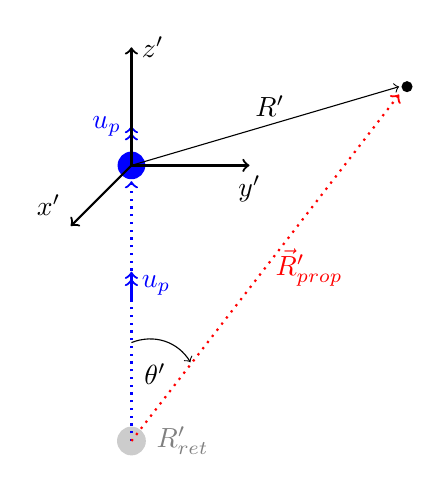
\begin{tikzpicture}[scale=5]
\draw[blue, thick,->>] (-0,0.36,0) -- (-0,0.43,0) node[midway, right]{$\Vec{u}_p$};
\draw[blue, thick,->>] (0,0.7,0) -- (0,0.8,0) node[left]{$\Vec{u}_p$};
\fill (0.7,0.9,0) circle (0.4pt);
\fill[blue] (0,0.7,0) circle (1pt);
\draw[gray!40,fill=gray!40] (0,0,0) circle (1pt);
\node[gray] at (0.13,0,0) {$\Vec{R}'_{ret}$};
\draw[black, thick,->] (0,0.7,0) -- (0.3,0.7,0) node[anchor=north]{$y'$};
\draw[black, thick,->] (0,0.7,0) -- (0,1,0) node[anchor=west]{$z'$};
\draw[black, thick,->] (0,0.7,0) -- (0,0.7,0.4) node[anchor=south east] {$x'$};
\node at (0.06,0.17,0) {$\theta '$};
\draw[->] (0,0.25,0) to[bend left=40] (0.15,0.2,0);
\draw[thick,blue,dotted,->] (0,0,0) -- (0,0.66,0);
\draw[red, thick, dotted,->] (0,0,0) -- (0.68,0.88,0) node[midway, right] {$\vec{R}'_{prop}$};
\draw[black,->] (0,0.7,0) -- (0.68,0.9,0) node[midway,above] {\text{ $\Vec{R}'$}};
\end{tikzpicture}
\caption{The diagram shows a particle $p$ in blue, moving at a velocity $\Vec{u}_p$, currently positioned at the origin of an axis, it shows light from the source that is currently at a position $\Vec{R'}$, this light has propagated from the source when it was at position $\Vec{R}'_{ret}$ in grey, this light had propagated from this retarded position, along $\Vec{R}'_{prop}$, shown in red, to get to its current position, at an angle of $\theta '$ to the Z-axis.  }
\label{fig: Retarded field outward field}
\end{figure}

As visualised in figure (\ref{fig: Retarded field outward field}). If we have a light source particle $p$, that is moving at velocity $\vec{u_p}=(0,0,u_p)$ along the Z-axis and is currently positioned at the origin of an axis at time $t'=0$ (here we are choosing to show it as a primed coordinate, but we are just preemptively doing this because it will make it easier to introduce the Lorentz transformations later, at the moment we are staying in the same frame and not special relativity is being used). then if we have light that has been propagated from the source to the coordinate $\Vec{R}'= (x',y',z')$ at this time, this light would of had to been emitted from $P$ at a previous/retarded point in time $T'_{ret}$, at a retarded coordinate $\Vec{R'}_{ret}= \Vec{u}_p T'_{ret}=(0,0,u_p T'_{ret})$, such that the light has propagated along

\begin{equation}%%%%%%%%%%%%%%%
\label{displacement}
    \Vec{R'}_{prop} = -\Vec{c}'T'_{ret} = \Vec{R'} - \vec{R}'_{ret} =  \begin{pmatrix}
    x'\\ y' \\ z' - u_p T'_{ret}
    \end{pmatrix},
\end{equation}%%%%
to $\Vec{R'}$.

To find this retarded time, we will start with the magnitude of the propagation displacement from previous equation which is equal to the distance the light, propagating at the speed of light, $c$, travels in the corresponding propagation time $T'_{prop}=-T'_{ret}$. This gives

\begin{equation}%%%%%%%%%%%%%%%
        \begin{aligned}
        \left( c T_{prop}'\right)^2  = \left( -c T_{ret}'\right)^2 &= \|\Vec{R'}_{prop}\|^2 \\
        &= (x'^2 + y'^2 + z'^2) + u_p^2 T_{ret}'^2 - 2u_p z' T_{ret}',
%        (c^2 - v^2) T_{ret}'^2 &=  (x'^2 + y'^2 + z'^2) + 2v T_{ret}'z'
        \end{aligned}
\end{equation}%%%%

rearranging this, we get the quadratic

\begin{equation}%%%%%%%%%%%%%%%
        T_{ret}'^{2} + \left(2\gamma^2\frac{u_p}{c^2} z'\right)T_{ret}' - \frac{\gamma^2}{c^2}(x'^2+y'^2+z'^2) = 0,
\end{equation}%%%%

where $\gamma = (1 - u_p^2/c^2)^{-1/2}$, we may be preemptively using the constant $\gamma$ here but we have still not used any special relativity. Now taking the solution for the past time (negative solution) using the quadratic formula, and making use of the identity

\begin{equation}%%%%%%%%%%%%%%%
\label{eq: gamma identity}
    \gamma^2 = 1+\gamma^2\frac{u_p^2}{c^2},
\end{equation}%%%%

we get the result

\begin{equation}%%%%%%%%%%%%%%%
\label{Retarded Time}
    \begin{aligned}
    T_{ret}' &= -\gamma^2\frac{u_p}{c^2}z' - \sqrt{\left(-\gamma^2\frac{u_p}{c^2} z'\right)^2+\frac{\gamma^2}{c^2}(x'^2+y'^2+z'^2)} \\
    &= -\gamma^2\frac{u_p}{c^2}z' - \frac{\gamma}{c}\sqrt{x'^2+y'^2+\left(1+\gamma^2\frac{u_p^2}{c^2}\right) z'^2}\\
    &= - \gamma^2\frac{u_p}{c^2}z' - \frac{\gamma}{c}\sqrt{x'^2+y'^2+\gamma^2 z'^2} \\
    &= - \gamma^2\frac{u_p}{c^2}z' - \frac{\gamma}{c}\|\vec{R}\|.
    \end{aligned}
\end{equation}%%%%

Now in the final step, we finally introduced special relativity, with the lorentz transform we requiring $t'= 0$ for all coordinates, meaning that the primed and proper axis overlap at this time, and taking the primed frame as moving at velocity $v=-u_p$ along the z-axis relative to the proper frame of particle, and hence used the Lorentz transform of the spatial coordinates; $\vec{R}=(x,y,z)=(x',y',\gamma z')$, to get $\|\vec{R}\|$. With this we can rewrite the Z-component of equation \eqref{displacement} as
\begin{equation}%%%%%%%%%%%%%%%
    z' - u_p T_{ret}' \Rightarrow \gamma\left(z + \frac{u_p\cdot \|\vec{R}\|}{c}\right),
\end{equation}%%%%
giving the propagation displacement vector to be
\begin{equation}%%%%%%%%%%%%%%%
\label{retarded displacement}
    \Vec{R}'_{prop}= \begin{pmatrix}
    x\\ y \\ \gamma \left(z + \dfrac{u_p \cdot \|\vec{R}\|}{c}\right)
    \end{pmatrix} = \|\vec{R}\|\begin{pmatrix}
    \frac{x}{\|\vec{R}\|}\\ \frac{y}{\|\vec{R}\|} \\ \gamma \left( \frac{z}{\|\vec{R}\|} + \dfrac{u_p}{c} \right)\\
    \end{pmatrix}.
\end{equation}%%%%
Since the light propagates along this in the primed frame, the unit vector of the primed propagation velocity at any general primed coordinate can be worked out to be (show working out in appendix)
\begin{equation}%%%%%%%%%%%%%%%
\label{eq: unit retarded velocity}
    \hat{\mathbf{\vec{U}'}} = \hat{\mathbf{\vec{R}'}}_{prop} = \dfrac{1}{\text{\AA}} \begin{pmatrix}
    \frac{x}{\|\vec{R}\|}\\ \frac{y}{\|\vec{R}\|} \\ \gamma \left( \frac{z}{\|\vec{R}\|} + \dfrac{u_p}{c} \right)
    \end{pmatrix},
\end{equation}%%%%
where the factor
\begin{equation}%%%%%%%%%%%%%%%
    \text{\AA} = \gamma\left( 1 + \frac{u_p}{c}\frac{z}{\|\vec{R}\|} \right).
\end{equation}%%%%
Now taking the magnitude of the light propagation displacement from equation \eqref{retarded displacement} and using equation \eqref{eq: gamma identity}, we have
\begin{equation}%%%%%%%%%%%%%%%
\label{eq: field displacement transform}
    \begin{aligned}
    \|\Vec{R}'_{prop}\|^2 &= x^2+y^2 + \gamma^2\left( z^2 +\frac{u_p^2}{c^2}\|\vec{R}\|^2 + 2 \frac{u_p}{c}z \|\vec{R}\| \right) \\
    &= \gamma^2 \|\vec{R}\|^2 + \frac{u_p^2}{c^2}\gamma^2z^2 + 2 \frac{u_p}{c}\gamma^2 z \|\vec{R}\| \\
    &= \gamma^2\left( \|\vec{R}\| + \frac{u_p}{c}z \right)^2\\
    &= \gamma^2\left( 1 + \frac{u_p}{c}\frac{z}{\|\vec{R}\|} \right)^2 \|\vec{R}\|^2 \\
    &= \text{\AA}^2 \|\vec{R}\|^2
    .
    \end{aligned}
\end{equation}%%%%
Since the luminal speed of the propagation will be same in both frames we have
\begin{equation}%%%%%%%%%%%%%%%
\label{eq: retarded field displacement transform}
\begin{aligned}
   c = \frac{\|\Vec{R}\|}{T_{prop}} &= \frac{\|\Vec{R}'_{prop}\|}{T_{prop}'}\\
    &=  \frac{\text{\AA}\|\Vec{R}\|}{T_{prop}'} \\
    T_{prop}' &= \text{\AA} T_{prop},
\end{aligned}
\end{equation}%%%%

where $T_{prop}$ is the proper (particles rest frame) time the light takes to propagate to $\vec{R}$ from the particle.

... is this correct to say?... Time and length are stretched in the primed frame along $\vec{R}'_{ret}$ relative to the proper frame along $\vec{R}$ by a factor $\text{\AA}$, leading to the relative radial density of the light in the primed frame to that of the proper frame, which we will refer to as the radial light strength weighting, given as
\begin{equation}%%%%%%%%%%%%%%%
\label{eq: radial weighting}
    W_\rho = \frac{1}{\text{\AA}}.
\end{equation}%%%%

%███████████████████████████████████████████████████████████████████
%███████████████████████████████████████████████████████████████████
\section{Acceleration}
*** gotta check which theta  this is
\subsection{General Equation}

\begin{equation}%%%%%%%%%%%%%%%
    \vec{a'} = \dfrac{1}{\gamma^2}\left[ \vec{a_0}+\left(\dfrac{1}{\gamma}-1\right)\left(\vec{a_0}\cdot\hat{\vec{v}}\right)\hat{\vec{v}}\right]
\end{equation}%%%%

\subsection{Co-moving Charges}

\begin{equation}%%%%%%%%%%%%%%%
    \vec{v} =  \begin{pmatrix}
    o\\
    v
    \end{pmatrix} =
    \begin{pmatrix}
    o\\
    -u_p
    \end{pmatrix}
\end{equation}%%%%

\begin{equation}%%%%%%%%%%%%%%%
    \vec{a_0} = \dfrac{k}{R^2} \begin{pmatrix}
    \sin\theta\\
    \cos{\theta}
    \end{pmatrix}
\end{equation}%%%%
Substituting into general equation

\begin{equation}%%%%%%%%%%%%%%%
    \vec{a'} = \dfrac{1}{\gamma^3}\dfrac{k}{R^2}\left[ \begin{pmatrix}
    \gamma\sin\theta\\
     \cos{\theta}
    \end{pmatrix} \right]
\end{equation}%%%%
\begin{equation}%%%%%%%%%%%%%%%
    \begin{aligned}
   \|\vec{a}'\| &=  \dfrac{1}{\gamma^2}\dfrac{k}{R^2}\sqrt{
    \sin^2\theta +
     \gamma^{-2}\cos^2{\theta}} \\
     &=  \dfrac{1}{\gamma^2}\dfrac{k}{R^2} \sqrt{
    \sin^2\theta +
     (1-\beta^2)\cos^2{\theta}} \\
     &=  \dfrac{1}{\gamma^2}\dfrac{k}{R^2} \sqrt{
    1 -\beta^2\cos^2{\theta}}
    \end{aligned}
\end{equation}%%%%
using trigonometry and retarded distance transform from above

\begin{equation}%%%%%%%%%%%%%%%
    \begin{aligned}
   \|\vec{a}'\| &=  \dfrac{1}{\gamma^2}\dfrac{k}{R^2} \sqrt{1 -\beta^2\cos^2{\theta}}\\
   &= \dfrac{1}{\gamma^2}\dfrac{k}{R^2} \sqrt{1 -\beta^2 \dfrac{(\cos\theta' + \beta)^2}{(1+\beta\cos\theta')^2}}\\
   &= \dfrac{1}{\gamma^2}\dfrac{k}{R^2} \sqrt{  \dfrac{(1+\beta\cos\theta')^2 - \beta^2(\cos\theta' + \beta)^2}{(1+\beta\cos\theta')^2}}\\
   &= \dfrac{1}{\gamma^2}\dfrac{k}{R^2} \sqrt{  \dfrac{(1+2\beta\cos\theta') - \beta^2(\beta^2 + 2 \beta\cos\theta')}{(1+\beta\cos\theta')^2}}\\
   &= \dfrac{1}{\gamma^2}\dfrac{k}{R^2} \sqrt{  \dfrac{(1-\beta^2)2\beta\cos\theta' + (1 - \beta^4)}{(1+\beta\cos\theta')^2}}
    \end{aligned}
\end{equation}%%%%

\begin{equation}%%%%%%%%%%%%%%%
\begin{aligned}
\vec{a'} &= \dfrac{1}{\gamma^3( 1+\beta\cos\theta')} \dfrac{k}{R^2} \begin{pmatrix}
    \sin\theta' \\
     \cos\theta' + \beta
    \end{pmatrix}\\
    &= \dfrac{1}{\gamma^3( 1+\beta\cos\theta')} \dfrac{k\left(\gamma\left(1+\beta\cos\theta^{'}\right)\right)^{-2}}{{R'_{ret}}^2} \begin{pmatrix}
    \sin\theta' \\
     \cos\theta' + \beta
    \end{pmatrix}\\
    &= \dfrac{1}{\gamma^5( 1+\beta\cos\theta')^3} \dfrac{k}{{R'_{ret}}^2} \begin{pmatrix}
    \sin\theta' \\
     \cos\theta' + \beta
    \end{pmatrix}
\end{aligned}
\end{equation}%%%%

\begin{equation}%%%%%%%%%%%%%%%
    \begin{aligned}
   \|\vec{a'}\| &=  \dfrac{1}{\gamma^3( 1+\beta\cos\theta')} \dfrac{k}{R^2}
    \sqrt{\sin^2\theta' + (\cos\theta' + \beta)^2} \\   &= \dfrac{1}{\gamma^3( 1+\beta\cos\theta')} \dfrac{k}{R^2}
    \sqrt{ 1 + \beta^2 +  2\cos\theta'\beta}
    \end{aligned}
\end{equation}%%%%

%███████████████████████████████████████████████████████████████████
%███████████████████████████████████████████████████████████████████
\section{Derivation from Spherical Light Pulse} \label{spherical light pulse derivation}%%%%%%%%%%%%%

*** what about reverse of the spherical wave derivation, so that the spherical pulse of light is emitted towards the origin to reach at time $t=0=t'$ (then it would be as if was emitted into the past if we continue the the propagation back through the origin)

***
If you have a point $r$ in an inertial frame then a spherical wave pulse would take $t= |r|/c$ to get there, we will call the light being at coordinate $r$ an event, now to find the corresponding event in the primed frame

*** free to choose the origin of the primed frame, so choosing it to be coinciding at the point light is emitted

***
maybe derive from spherical pulse on lorry, having it return and have its walls be general coordinates, with time dilation

*** derivation in words first:
- 2 inertial frames coinciding at $t=t'=0$ with primed frame moving relativity in z-direction
- Describe spherical wave pulse in proper frame and primed frame $|\vec{R}|=ct$ and $|\vec{R'}|=ct'$
-

...

An observer is at the origin of an inertial frame of reference/coordinate system $<S>$. An object moving at a constant velocity $v$ relative to $<S>$ can be described to be stationary in an inertial frame of reference $<S'>$ moving the at the same velocity $v$ shown in Fig. \ref{ltrans}.

\begin{figure}[ht]
\begin{tikzpicture}[scale=3]%,tdplot_main_coords]
\coordinate (O) at (0,0,0);
%
\draw (0,2,0) node{$t=0$};
\draw (-0.8,2,0) node{ {\large $<S>$}};
\draw[black, thick,->] (-0.2,0,0) -- (0.8,0,0) node[anchor=north east]{$x$};
\draw[black, thick,->] (0,-0.2,0) -- (0,0.8,0) node[anchor=north west]{$z$};
\draw[black, thick,->] (0,0,0.3) -- (0,0,-1) node[anchor=south]{$y$};
\draw[gray,dashed, thick,->] (-0.2,0,0) -- (0.4,0,0) node[anchor=north east]{$x'$};
\draw[gray,dashed, thick,->] (0,-0.2,0) -- (0,0.4,0) node[anchor=south west]{$z'$};
\draw[gray,dashed, thick,->] (0,0,0.3) -- (0,0,-0.5) node[anchor=south]{$y'$};
\draw[gray, thick, ->>] (-0.15,0,0) -- (-0.15,0.22,0) node[anchor=east]{$v$};
\fill[red] (0.65,0.2,0) circle (0.6pt);
\draw[gray, thick, ->>] (0.65,0.2,0) -- (0.65,0.42,0) node[anchor=west]{$v$};
%
\draw (1.7,2,0) node{$t>0$};
\draw[black, thick,->] (1.5,0,0) -- (2.5,0,0) node[anchor=north east]{$x$};
\draw[black, thick,->] (1.7,-0.2,0) -- (1.7,0.8,0) node[anchor=north west]{$z$};
\draw[black, thick,->] (1.7,0,0.3) -- (1.7,0,-1) node[anchor=south]{$y$};
%
\draw[gray, dashed, thick,->] (1.5,1.2,0) -- (2.2,1.2,0) node[anchor=north east]{$x'$};
\draw[gray, dashed, thick,->] (1.7,1,0) -- (1.7,1.7,0) node[anchor= west]{$z'$};
\draw[gray, dashed, thick,->] (1.7,1.2,0.3) -- (1.7,1.2,-0.8) node[anchor=south]{$y'$};
\draw[gray, thick, ->>] (1.55,1.2,0) -- (1.55,1.42,0) node[anchor=east]{$v$};
\fill[red] (2.35,1.4,0) circle (0.6pt);
\draw[gray, thick, ->>] (2.35,1.4,0) -- (2.35,1.62,0) node[anchor=west]{$v$};
%
\end{tikzpicture}
\caption{Proper frame of reference in standard configuration.}
\label{ltrans}
\end{figure}

\begin{figure}[H]
\begin{tikzpicture}[scale=3]%,tdplot_main_coords]
\coordinate (O) at (0,0,0);
%
\draw (0,1,0) node{$t'=0$};
\draw (-0.8,1,0) node{ {\large $<S'>$}};
\draw[black, thick,->] (-0.2,0,0) -- (0.8,0,0) node[anchor=north east]{$x'$};
\draw[black, thick,->] (0,-0.2,0) -- (0,0.8,0) node[anchor=north west]{$z'$};
\draw[black, thick,->] (0,0,0.3) -- (0,0,-1) node[anchor=south]{$y'$};
\draw[gray,dashed, thick,->] (-0.2,0,0) -- (0.4,0,0) node[anchor=north east]{$x$};
\draw[gray,dashed, thick,->] (0,-0.2,0) -- (0,0.4,0) node[anchor=south west]{$z$};
\draw[gray,dashed, thick,->] (0,0,0.3) -- (0,0,-0.5) node[anchor=south]{$y$};
\draw[gray, thick, ->>] (-0.15,0,0) -- (-0.15,-0.22,0) node[anchor=east]{$-v$};
\fill[red] (0.65,0.4,0) circle (0.6pt);
\fill[red] (2.35,0.4,0) circle (0.6pt);
%
\draw (1.7,1,0) node{$t'>0$};
\draw[black, thick,->] (1.5,0,0) -- (2.5,0,0) node[anchor=north east]{$x'$};
\draw[black, thick,->] (1.7,-0.2,0) -- (1.7,0.8,0) node[anchor=north west]{$z'$};
\draw[black, thick,->] (1.7,0,0.3) -- (1.7,0,-1) node[anchor=south]{$y'$};
%
\draw[gray, dashed, thick,->] (1.5,-0.9,0) -- (2.2,-0.9,0) node[anchor=north east]{$x$};
\draw[gray, dashed, thick,->] (1.7,-1.1,0) -- (1.7,-0.4,0) node[anchor= west]{$z$};
\draw[gray, dashed, thick,->] (1.7,-0.9,0.3) -- (1.7,-0.9,-0.8) node[anchor=south]{$y$};
\draw[gray, thick, ->>] (1.55,-0.9,0) -- (1.55,-1.12,0) node[anchor=east]{$-v$};
%
\end{tikzpicture}
\caption{Primed frame of reference in standard configuration.}
\end{figure}

\begin{itemize}
\setlength\itemsep{0em}

\item We start with setting the inertial frames up so that the origins of the Cartesian coordinates coincide at $t=0=t'$

\item It is chosen that the frame of reference $<S'>$ moves in the z-direction (this is chosen as it is easier to move to spherical polar coordinates later and since there is symmetry in the coordinates perpendicular to the movement, and having right-left symmetry is more visually simple)

\item *** if there is a spherical light pulse at the time the coordinate axis overlap at $t=t'=0$ such that the distance that the light has propagated at a time $t$ is $ct$ and $ct'$ respectfully so that the equation describing the spherical pulse in each frame is $ct = \sqrt{ x^2 + y^2 + z^2 }$ and $ct' = \sqrt{ x'^2 + y'^2 + z'^2 }$

\item We define the $s$ and $s'$ as:

\vspace{-1cm}
\begin{equation}%%%%%%%%%%%%%%%
\begin{aligned}
 s^2 &= -c^2t^2 + x^2 + y^2 + z^2 \\  s'^2 &= -c^2t'^{2} + x'^2 + y'^2 + z'^2
\end{aligned}
\label{s}
\end{equation}%%%%

*** Diagram of wave fronts with both axis in same diagram one moving relative to other showing  (maybe having 2 diagrams one with each frame of reference at rest) ***

\item At an expanding wave front moving at the speed of light $c$, in the two frames we have $s= s'=0$

\item We are therefore looking for a transformation s.t. $s=0 \Leftrightarrow s'=0$

\item for a linear transform it is implied $s'^2= k s^2$ (where k is a constant) ** why does it have to be linear? (to allow for smooth inverse transformation)

\item By symmetry $ s^2=k^2 s'^2=k^2 s^2$ which leads to $ k^2= 1 \Rightarrow k=1$ ( $k=-1$ is disallowed because as $v\rightarrow 0$ we must recover $s=s'$ )

\item So $s'^2=s^2$, and by symmetry $x'=x$, $y'=y$ (this is taken from the cannon and ball thought experiment from chapter...)

\item This leads to:
\vspace{0cm}
\begin{equation}%%%%%%%%%%%%%%%
\label{seqs}
-c^2t^2+ z^2 = -c^2t'^2 +z'^2
\end{equation}%%%%

\item The requirement $z'=0$ when $z=vt$, the form of a linear equation that gives this for all values of $t$ is
\vspace{0cm}
\begin{equation}%%%%%%%%%%%%%%%
\label{xbar}
z' = \gamma (z-vt)
\end{equation}%%%%
\item where $\gamma$ is yet to be determined, we have chosen the linear equation and not one that depends on factors greater than first order, i.e. squared or greater terms of $(z-vt)$, this is because the linear... (to allow for smooth inverse transformation)

\item By symmetry if we wanted to instead transform from $<S'>$ to $<S>$, it is the same transform but with the frame change in the opposite direction, so $x,y,z,t$ can just be replaced by $x',y',z',t'$ when the sign in front of $v$ is also changed *** maybe diagram to show this

\item Substituting $z'$ into the inverse of eq. \eqref{xbar} leads to

\begin{equation}%%%%%%%%%%%%%%%
\label{ttrans}
    t'=\gamma \bigg[t-\frac{z}{v}\bigg(1-\frac{1}{\gamma^2}\bigg)\bigg]
\end{equation}%%%%

\item Subbing the previous two equations into eq. \eqref{seqs} gives

\begin{equation}%%%%%%%%%%%%%%%
    -c^2t^2+ z^2 = -c^2\gamma^2\bigg[ t -\frac{z}{v}\bigg(1-\frac{1}{\gamma^2}\bigg)\bigg]^2 + \gamma^2(z-vt)^2
\end{equation}%%%%

\item This holds true for all $z$ and $t$
\item Equating terms ( this is a mathematical technique, were it is known that for an equation like this to be true for all values of $t$ it is required that all terms in front $t^2$ on each side of the equation must be equal) in front of $t^2$ leads to

\begin{equation}%%%%%%%%%%%%%%%
\mhl{
    \gamma= \frac{1}{\sqrt{1-\beta^2}}
    }
\end{equation}%%%%

\item Subbing this into previous equations now completes the Lorentz Transformation:

%\vspace{-1cm}
\begin{equation}%%%%%%%%%%%%%%%
\label{lorentz transformation 2}
\mhl{
    \begin{aligned}
      &  x'=x \\ & y'=y \\ &z' = \gamma (z-vt)  \\
       \text{From eq. \eqref{ttrans} \ \ \ } & t'=\gamma \bigg(t-\frac{vz}{c^2}\bigg)
    \end{aligned}
    }
\end{equation}%%%%
*** explain the time transform in terms of the gamma function being the slowing down part and the $\frac{vz}{c^2}$ being the "anti-simultaneity" part
%\vspace{-0.9cm}
\item Galilean coordinates obtained by letting $v\rightarrow 0$
\end{itemize}
we can write this in vector form, multiplying $t'$ by $c$ to give unit of length, this is known as the positional 4 vector and is given as
\begin{equation}%%%%%%%%%%%%%%%
\label{spacial transform}
    \bf{R}'= \begin{pmatrix}
    ct' \\ x'\\ y' \\ z'
    \end{pmatrix} = \begin{pmatrix}
    \gamma\left( ct - \dfrac{vz}{c} \right) \\x\\ y \\ \gamma \left( z - vt \right)\\
    \end{pmatrix}.
\end{equation}%%%%
an event is given by its spacial coordinates and the time at which it happens.

%███████████████████████████████████████████████████████████████████
\section{Length Contraction}
%███████████████████████████████████████████████████████████████████
\section{Time Dilation}

Taking two times $t_1$ and $t_2$ of a clock at rest at position $z$ in one inertial frame will have transformed times in another reference frame of $t'_1 = \gamma(t_1 - \frac{v}{c^2}z_1)$ $t'_2 = \gamma(t_2 - \frac{v}{c^2}z_2)$ so that the difference in time is

\begin{equation}%%%%%%%%%%%%%%%
\begin{aligned}
   \Delta t' &=  t'_2 - t'_1 \\ &= \gamma(t_2 - \frac{v}{c^2}z) - \gamma(t_1 - \frac{v}{c^2}z) \\ &= \gamma (t_2 - t_1 ) \\ &= \gamma \Delta t
\end{aligned}
\end{equation}%%%%
when we take the change of time at the same location in a rest frame, we always have that $\Delta t' > \Delta t$ i.e the change in time in the rest frame of an observer corresponds to a greater change in time in another moving frame of reference.

%███████████████████████████████████████████████████████████████████
%███████████████████████████████████████████████████████████████████
\section{Generalised velocity vector transform}
%███████████████████████████████████████████████████████████████████
\subsection{god knows what this is: Doppler Effect}

%██████████
\begin{figure}[ht]
\begin{subfigure}{.49\textwidth}
  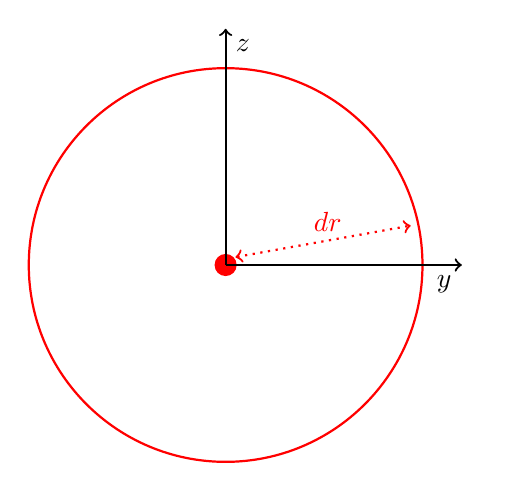
\begin{tikzpicture}[scale=5]
\draw[white] (0,0.6,0) -- (0,-0.5,0);
\draw[white] (0.7,0) -- (-0.5,0);
\fill[red] (0,0,0) circle (0.8pt);
\draw[red,thick] (0 ,0) circle (0.5);
\draw[black, thick,->] (0,0,0) -- (0.6,0,0) node[anchor=north east]{$y$};
\draw[black, thick,->] (0,0,0) -- (0,0.6,0) node[anchor=north west]{$z$};
%\draw[->] (0,0.25/2,0) to[bend left=45] (0.21/2,0.04,0);
%\node at (0.08,0.17,0) {$\theta $};
\draw[red,thick, dotted,<->] (0.025,0.02,0) -- (0.47,0.1,0) node[midway,above] {\text{ $dr$}};
\end{tikzpicture}
\caption{Spherical pulse in rest frame}
%  \label{fig:sub1}
\end{subfigure}
\begin{subfigure}{.49\textwidth}
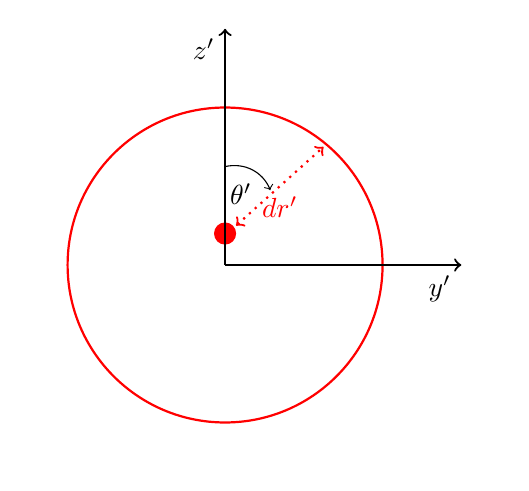
\begin{tikzpicture}[scale=5]
\draw[white] (0,0.6,0) -- (0,-0.5,0);
\draw[white] (0.7,0) -- (-0.5,0);
\fill[red] (0,0.08,0) circle (0.8pt);
\draw[red,thick] (0 ,0) circle (0.4);
\draw[thick,->] (0,0,0) -- (0.6,0,0) node[anchor=north east]{$y'$};
\draw[thick,->] (0,0,0) -- (0,0.6,0) node[anchor=north east]{$z'$};
\draw[red,thick, dotted,<->] (0.028,0.1,0) -- (0.25,0.3,0) node[midway, below] {$dr'$};
\draw[->] (0,0.25,0) to[bend left=40] (0.23/2,0.19,0);
\node at (0.04,0.18,0) {$\theta' $};
\end{tikzpicture}
\caption{Spherical pulse in Primed frame}
%  \label{fig:sub2}
\end{subfigure}
\caption{ since I have everything in opposite directions, need to change equations *** also this is full blown relativity not just retarded field }
\label{fig: Doppler effect appendix}
\end{figure}
%██████████
**** this is for receiving particle that is at rest, i.e. $u_p=0$ ****

Figure (\ref{fig: Doppler effect appendix}), shows a particle emitting a spherical wave of light, in the proper frame it begins emitting at time $t=0$ and after an infinitesimal amount of time the front of the wave has spread out spherically, such that the front is at a distance $dr$ from the origin at all positions,while the wave continues to be emitted from the origin. In the primed frame the wavefront is emitted at $t'=0$ and reaches a point that is $\gamma dr$ from the origin at all points, with the gamma due to $dr=cdt$ and the the time $dt=\gamma dt'$, but we also now have to take into account that the source particle that is still emitting this wave has moved along the z'-axis to a point $u_p dt'= \gamma u_p dt$ and each part of the wave being emitted from the source is taken as being emitted at an angle $\theta'$, such that any point on the wavefront that is at and angle of $\theta'$ from the particle, will have the distance $dr'$ between it and the source, and the wave that is currently being emitted from the source particle will go to that position on the wavefront (offal description).

We can get the Doppler effect by taking the ratio of the distances the way will have to travel to get to the current point the wavefront is at, which in the rest frame is $dr=cdt$ and in the primed frame is $|d\vec{dr}'| = u_p/c \gamma dr$

%███████████████████████████████████████████████████████████████████
%███████████████████████████████████████████████████████████████████
\chapter{Velocity Transformation Alternative Derivation}
*** diagram *** \newline
The change in position of particle $\Delta \mathbf{R}_p$, with initial position $\mathbf{R}_0$, and a constant velocity
\begin{equation}%%%%%%%%%%%%%%%
    \mathbf{U}_p = \begin{pmatrix}
        u_x \\ u_y \\ u_z \\
    \end{pmatrix}
\end{equation}%%%%
between time $t_1$ and $t_2$ is
\begin{equation}%%%%%%%%%%%%%%%
    \Delta \mathbf{R}_p = (\mathbf{R}_0 +\mathbf{U}_p t_2) - (\mathbf{R}_0 +\mathbf{U}_p t_1) =  (t_2 - t_1) \mathbf{U}_p =  \mathbf{U}_p \Delta t
\end{equation}%%%%
(acceleration as well, but these will become negligible when we take an infinitesimal time interval later)
The \hyperlink{def-lorentz-transform}{Lorentz transformation} for this with $t=0$ is
\begin{equation}%%%%%%%%%%%%%%%
    \Delta \mathbf{R}'_p = \begin{pmatrix}
        u_x \Delta t \\ u_y \Delta t \\ \gamma \left( u_z \Delta t - v \Delta t \right) \\
    \end{pmatrix}
\end{equation}%%%%
but this gives primed times to be $\Delta t'=-\gamma\dfrac{v}{c^2} u_z \Delta t$, and we want to find the positions that have the same time, therefore we need to take away the displacement moved in the the primed time $\Delta t' \mathbf{U'}_p $ which is
\begin{equation}%%%%%%%%%%%%%%%
    \Delta \mathbf{R}'_p = \begin{pmatrix}
        u_x \Delta t \\ u_y \Delta t \\ \gamma \left( u_z \Delta t - v \Delta t \right) \\
    \end{pmatrix} + \gamma\dfrac{v}{c^2} u_z \Delta t  \mathbf{U'}_p.
\end{equation}%%%%
If we divide across by the change in time $\Delta t$ and take this time change to go to an infinitesimal $dt$ and substituting the time in terms of \hyperlink{def-time-dilation}{dilated primed time} $dt = \frac{1}{\gamma}dt'$ we then have the primed velocity given as *** the dt' = gamma dt is suspicious ***
\begin{equation}%%%%%%%%%%%%%%%
    \dfrac{d \mathbf{R}'_p}{dt} =\gamma \dfrac{d \mathbf{R}'_p}{dt'} = \gamma\mathbf{U'}_p   = \begin{pmatrix}
        u_x \\ u_y  \\ \gamma \left( u_z  - v  \right) \\
    \end{pmatrix} + \gamma\dfrac{v}{c^2} u_z  \mathbf{U'}_p
\end{equation}%%%%
rearranging for primed velocity we have
\begin{equation}%%%%%%%%%%%%%%%
    \mhl{
        \begin{aligned}
            & \mathbf{U'}_p = \dfrac{1}{\gamma\left(1- \dfrac{v}{c^2} u_z\right) }\begin{pmatrix}
               u_x \\ u_y  \\ \gamma \left( u_z  - v  \right) \\
            \end{pmatrix} \\
            & \text{at position $\mathbf{R'}$ and time $t'$ }
        \end{aligned}
    }
\end{equation}%%%%
%███████████████████████████████████████████████████████████████████
%███████████████████████████████████████████████████████████████████
\chapter{Todo for these notes}
* \AA \ \ is not the same \AA \ \ in velocity and acceleration transform as it is in time transform (( it is the same as its the retarded cosine angel which is same as cosine of angle for primed frame as its at the retarded position

(try to make it as readable as possible for people with poor English, or for the translation)

an introduction sentence... ((relativity cause its the theory of motion for objects relative to other objects, and special because its specifically for the special case where gravity's effects negligible and are not required to be included in calculations and objects are moving at constant velocities)) ((as gravity curves spacetime giving curved coordinates))

decide whether to include minkowski diagram as it is an abstract view rather than representational view

%███████████████████████████████████████████████████████████████████
%███████████████████████████████████████████████████████████████████
\section{A note on different notations}
*primed notation
* my notation for frames

3 postulates/ starting points.

%███████████████████████████████████████████████████████████████████
\section{Astronomy from Earth}

... explain how observation from earth works, as you would think the positions of stars at $t'=0$ would be all over the place as it rotates around the sun

%███████████████████████████████████████████████████████████████████
%███████████████████████████████████████████████████████████████████
\section{Four Acceleration}

...proper acceleration. differentiate the velocity invariant quantity, it will give \( \frac{d^2 S}{d\tau^2} = 0 = ...\frac{d^2 S}{dt{'}^2} \)

... this is bad math explaination using square of derivative

need to use the square quantity not singular

\begin{equation}
	\begin{aligned}
		\frac{d}{d\tau} \left(\frac{dS_p}{d\tau}\right)^2 & = \left(\frac{d}{d\tau}\right)^2 \left[ \left(c\gamma_{u}\right)^2-\left(u\gamma_{u} \right)^2 \right]                           \\
		\frac{1}{2} \frac{dS_p}{d\tau} \frac{d^2S_p}{d\tau^2}                               & = \gamma_u^2\left(\frac{d}{dt}\right)^2 \left[ \left(c\gamma_{u}\right)^2-\left(u\gamma_{u} \right)^2 \right]                           \\
		                                                              0   & = \gamma_u^2\left(c\frac{d \gamma_{u}}{dt}\right)^2-\gamma_u^2\left(\frac{d\left(u\gamma_{u} \right)}{dt}\right)^2 \\
																	  & = \gamma_u^2 \left( \gamma_u^3 \frac{u a}{{c}^2} \right)^2-\gamma_u^2\left( \gamma_u^3 a \right)^2
	\end{aligned}
\end{equation}

... this is more complex and one difference in this 4-vector here is that the spatial part of the 4-acceleration is not parallel to the 3-acceleration in a \hyperlink{def-Primed-Frame}{primed frame}

\begin{equation}
	\mathbf{A} = {\gamma}_{u}^4
	\begin{pmatrix}
		-c\frac{\mathbf{a}\cdot\mathbf{u}}{{c}^2}                                  \\
		\frac{1}{{\gamma}_{u}^2} {{a}_{x}}-{{u}_{x}} \frac{\mathbf{a}\cdot\mathbf{u}}{{c}^2} \\
		\frac{1}{{\gamma}_{u}^2} {{a}_{y}}-{{u}_{y}} \frac{\mathbf{a}\cdot\mathbf{u}}{{c}^2} \\
		\frac{1}{{\gamma}_{u}^2} {{a}_{z}}-{{u}_{z}} \frac{\mathbf{a}\cdot\mathbf{u}}{{c}^2} \\
	\end{pmatrix}
\end{equation}

this is not really the same thing as what we think of when we think of acceleration, as it does not give the rate of change of velocity in the normal sense in 3d space

\begin{equation}
	\begin{aligned}
		A & = \dfrac{dV}{d\tau} =
		\dfrac{dt}{d\tau}\cdot\dfrac{dV}{dt}                                                                                                                                   \\
		  & = \dfrac{dt}{d\tau}\cdot \dfrac{d}{dt}
		\left(\begin{array}{*{20}{c}} {\gamma}_{u}{c}\\ {\gamma}_{u} u \\ 0 \\ 0 \end{array}\right)
		 = {\gamma}_{u}
		\left(\begin{array}{*{20}{c}} \dfrac{u}{c}\;{\gamma}_{u}^3\;a \\ \dfrac{u^2}{{c}^2}\;{\gamma}_{u}^3\;a + {\gamma}_{u} a \\ 0 \\ 0 \end{array}\right) \\
		  & =
		\left(\begin{array}{*{20}{c}} \dfrac{u}{c}\;{\gamma}_{u}^4\;a \\ {\gamma}_{u}^2\left(\dfrac{u^2}{{c}^2}\;{\gamma}_{u}^2 + 1\right)a \\ 0 \\ 0 \end{array}\right)
		 = {\gamma}_{u}^4\;a
		\left(\begin{array}{*{2}{c}} \dfrac{u}{c} \\ 1 \\ 0 \\ 0 \end{array}\right)
	\end{aligned}
\end{equation}

%███████████████████████████████████████████████████████████████████
%███████████████████████████████████████████████████████████████████
\section{Force}

\begin{equation}
	\mathbf{F} = \frac{d\mathbf{p}}{d\tau} = m_0\mathbf{A}
\end{equation}

%███████████████████████████████████████████████████████████████████
\subsection{Force Transform}

*** one of the most confusing topics in special relativity, from the way it is defined, how it is derived, and how it relates to other things\newline

*** (a note that the 3-force in special relativity is specifically defined as the time derivative of momentum $\frac{d\mathbf{p}}{dt}$ and not mass times the acceleration $m\mathbf{a}$, this is due to newtons 2nd law holding only for the first definition in special relativity) \newline
*** This means that acceleration turns out not to be in the same direction as the force in special relativity\newline

force derivation is confusing as most sources give the time derivative of u and v as acceleration, (are they using that each force has opposite and equal force, but that would not take into account the retardedness)

\begin{equation}
	\mathbf{a} = \frac{1}{m_0 {\gamma}(\mathbf{v})} \left( \mathbf{F}-\frac{ ( \mathbf{v} \cdot \mathbf{F} ) \mathbf{v} }{{c}^2} \right)
\end{equation}

\begin{equation}
	\mathbf{F} = {\gamma}^3 m_0 \, \mathbf{a}_\parallel + {\gamma} m_0 \, \mathbf{a}_\perp
\end{equation}

%███████████████████████████████████████████████████████████████████
\subsection{not sure what this is}

The force parallel to the velocity of the \hyperlink{def-Primed-Frame}{primed frame} is unchanged, $\mathbf{F}_{\parallel \langle {'} \rangle} = \mathbf{F}_{\parallel}$, and the force perpendicular to this is $\mathbf{F}_{\perp \langle {'} \rangle} = {\gamma} \mathbf{F}_{\perp}$, with total force, $\mathbf{F} = \mathbf{F}_{\parallel} + \mathbf{F}_{\perp}$ and

\begin{equation}
	\mathbf{F}_{\parallel} = \dfrac{(\mathbf{F}\cdot\mathbf{v})}{\|\mathbf{v}\|^2}\mathbf{v}
\end{equation}

and substituting this into the formula for total force:

\begin{equation}
	\mathbf{F}_{\perp} = \mathbf{F}-\dfrac{(\mathbf{F}\cdot\mathbf{v})}{\|\mathbf{v}\|^2}\mathbf{v}
\end{equation}

since $\mathbf{F}_{\langle {'} \rangle} = \mathbf{F}_{\parallel \langle {'} \rangle} + \mathbf{F}_{\perp\langle {'} \rangle}$ we can use equations above to get:

\begin{equation}
	\begin{aligned}
		\mathbf{F}_{\langle {'} \rangle} & = \dfrac{(\mathbf{F}\cdot\mathbf{v})}{\|\mathbf{v}\|^2}\mathbf{v} + {\gamma}\bigg(\mathbf{F}-\dfrac{(\mathbf{F}\cdot\mathbf{v})}{\|\mathbf{v}\|^2}\mathbf{v}\bigg) \\
		                               & = {\gamma}\mathbf{F} + (1-{\gamma})\dfrac{(\mathbf{F}\cdot\mathbf{v})}{\|\mathbf{v}\|^2}\mathbf{v}
	\end{aligned}
\end{equation}

this is the same for the electric field as it only differs by some magnitude from the force.\newline
this is similar to how we get the reverse transform: (is it the primed velocity used in this?)

\begin{equation}
	\mathbf{F} = \dfrac{1}{{\gamma}}\mathbf{F}_{\langle {'} \rangle} + (1-\dfrac{1}{{\gamma}})\dfrac{(\mathbf{F}_{\langle {'} \rangle} \cdot\mathbf{v}_{\langle {'} \rangle} )}{\|\mathbf{v}_{\langle {'} \rangle} \|^2}\mathbf{v}_{\langle {'} \rangle}
\end{equation}

%███████████████████████████████████████████████████████████████████
%███████████████████████████████████████████████████████████████████
\section{Paradoxes and confusions:}

Before the discovery of Lorentz transformations the force was the same when it was defined by the multiplication of mass times acceleration or rate of change of momentum, but these two things are not equivalent when it comes to special relativity\\
So the force in special relativity was chosen to be by definition the later explanation (the rate of change of momentum)\\
This leaves us with the force not being in the same direction as the acceleration of an object in an inertial frame apart from some special cases, (i.e force and acceleration are in the direction velocity of the frame that we are transforming into)


%███████████████████████████████████████████████████████████████████
\section{"zitterbewegung"} \label{ch: "zitterbewegung"}

%███████████████████████████████████████████████████████████████████
\section{equation for motion in primed frame for arbitrary motion in proper frame} \label{ch: equation for motion in primed frame for arbitrary motion in proper frame}

%███████████████████████████████████████████████████████████████████
\section{None Point Like Sources} \label{ch: None Point Like Sources}
... and seeing moving objects rotated, i.e. can see the rear side of a cube before the rear side has moved past you

%███████████████████████████████████████████████████████████████████
\chapter{Thought Experiments} \label{ch: Thought Experiments}
Bell's Paradox and others
two identical particles that have a mass and charge such that in the frame where they are both at rest, such that the force of the gravitational attraction and the force of the electric repulsion cancel out, then in a frame where they are now both moving the forces still have to cancel, is there now a magnetic force, how does the gravitational field have to change. now what if they were instead rotating around the center of mass instead, with the gravity being the correct amount stronger such that there is this orbiting

... touch on GR, i.e. elevator thought experiment

Well we could have things be thinner if moving relative to the aether but not thinner between frames because observer also gets thinner as they are also moving relative to the aether at different speeds in each frame

%███████████████████████████████████████████████████████████████████
\chapter{Cheat Sheet} \label{ch: Cheat Sheet}

all needed equations
steps for tranforming between actuall positions and times
steps for transforming retarded positions and times

%███████████████████████████████████████████████████████████████████
%███████████████████████████████████████████████████████████████████
\section{Paths of Particles} \label{sect: Paths of Particles}

In an initial frame, we can describe the position at any time by the following generalized equations were the constants depend on the specific case

\begin{equation}
	\begin{aligned}
		 & x(t) = a_0 + a_1 t + a_2 t^2 + ... \\
		 & y(t) = b_0 + b_1 t + b_2 t^2 + ... \\
		 & z(t) = c_0 + c_1 t + c_2 t^2 + ...
	\end{aligned}
\end{equation}

then the corresponding primed equations are given as

\begin{equation}
	\begin{aligned}
		& {x{'}}(t) = x(t)                                         \\
		& {y{'}}(t) = y(t) \\
		& {z{'}}(t) = {\gamma} (z(t) - {v}{t})                       \\
	   \text{at time \ \ \ }                                   \\
		& {t{'}}(t) = {\gamma} \bigg(t-\frac{{v}}{{c}^2} z(t) \bigg)
   \end{aligned}
\end{equation}

with

\begin{equation}
	{t} = {\gamma} \left( t' + \dfrac{{v}{z'}}{{c}^2} \right)
\end{equation}

*** can not make x', y', z' in terms of primed time t'

\begin{equation}
		\begin{aligned}
			 & \mathbf{U}{'} = \dfrac{1}{{\gamma}\left(1-\dfrac{v}{{c}^2} {{u}_{z}}\right) }
			\begin{pmatrix}
				{{u}_{x}}                              \\
				{{u}_{y}}                              \\
				{\gamma} \left( {{u}_{z}}- {v} \right) \\
			\end{pmatrix}
			\\
			 & \text{at position ${\mathbf{r}{'}}$ and time ${t{'}}$ }
		\end{aligned}
\end{equation}

\begin{equation}
	{t{'}} = {\gamma} \bigg(t-\frac{{v}{z}}{{c}^2}\bigg)
\end{equation}

\begin{equation}
	{z} = {\gamma} ({z{'}}+{v}{t{'}})
\end{equation}


*** to be done,

may explain how it is not possible to derive how paths of a particle transforms into a second frame generally

try x,y,z all in terms of time T

try to give just what the aberrated/retarded path would look like i.e. transform retarded to retarded path

%███████████████████████████████████████████████████████████████████
%███████████████████████████████████████████████████████████████████
\section{Steps for Changing Frames} \label{sect: Steps for Changing Frames}

This section outlines the steps that should be taken to change between two inertial frames: \newline

Firstly let us talk about going from the retarded coordinates of objects in one frame to a second frame.
So if in your initial frame, you have an observer at rest at the origin, and different objects are moving around in this frame, if we take the retarded positions $\mathbf{r}_{ret}$ of the objects (i.e.
as the observer sees them positioned due to the delay in the light from the object), and use the retarded times of these objects which is ${t}_{ret} =-\frac{\|\mathbf{r}_{ret}\|}{c}$ with the coordinate transform, then these retarded positions in the initial reference frame will be transformed to their retarded positions in the second frame at their retarded times within it.
\newline

Another option is that you want to go from the object's positions that have times that are synchronized with the observer to positions that are also synced with the observer in the primed frame.
Then we need to start with all objects where they currently are at ${t} = 0$ then the coordinate transformation transforms the positions to the primed positions in the second frame, but at desynchronized times, so that we will have to propagate these objects forward or back in time until they are all at the time of the observer at the origin which is ${t{'}} = 0$ if the velocities of the objects are constant then you will only need to find their primed velocities, but if the initial frames velocities are not constant this is then a bit trickier, as you will have to worry about the transformations of acceleration to find its position at ${t{'}} = 0$.

%███████████████████████████████████████████████████████████████████
%███████████████████████████████████████████████████████████████████
%███████████████████████████████████████████████████████████████████
\chapter{differentials form light field}\label{ch: differentials form light field}

%███████████████████████████████████████████████████████████████████
\subsection{General Infintesmal Change in all Spatial Coordinates:}


now we will see what happens when we have an infintesmal change from an intial point $(x,y,z)$ to $(x_2,y_2,z_2)=(x +dx,y+dy,z+dz)$

two useful simifications we can do is first on $M$ for the point after the displacement we can use the taylor expansion to get

\begin{equation}
	\begin{aligned}
		M_2 &= \sqrt{(x+dx)^2 + (y+dy)^2 + \gamma_u^2 (z+dz)^2} \\
		&= \sqrt{x^2 + y^2 + \gamma_u^2 z^2} + \frac{xdx + ydy + \gamma^2 zdz}{\sqrt{x^2 + y^2 + \gamma_u^2 z^2}} \\
		&= M + \frac{xdx + ydy + \gamma^2 zdz}{M}
	\end{aligned}
\end{equation}

giving the change in $M$ as

\begin{equation}
	dM = M_2 - M = \frac{xdx + ydy + \gamma^2 zdz}{M}
\end{equation}

\begin{equation}
		cT_{p} - cT_{p2} = - \gamma_u^2 \frac{u}{c} dz - \gamma_u dM
\end{equation}

now from the light velocity unit vector we have

which gives

\begin{equation}
	\mathbf{\hat{c}}_2 - \mathbf{\hat{c}} = \mathbf{\hat{c}}_2 = \frac{1}{c T_{p2}}
	\begin{pmatrix}
		x_2 \\
		y_2 \\
		z_2 + u T_{p2}
	\end{pmatrix} - \frac{1}{c T_{p}}
	\begin{pmatrix}
		x \\
		y \\
		z + u T_{p}
	\end{pmatrix}
\end{equation}

\begin{equation}
	\mathbf{\hat{c}}_2 - \mathbf{\hat{c}} = \frac{1}{c T_{p} \cdot c T_{p2}}
	\begin{pmatrix}
		c T_{p} x_2 - c T_{p2} x\\
		c T_{p} y_2 - c T_{p2} y\\
		c T_{p} (z_2 + u T_{p2}) - c T_{p2} (z + u T_{p})
	\end{pmatrix}
\end{equation}

%███████████████████████████████████████████████████████████████████
\subsection{Infintesmal Change in $z$-direction:}

for only a infintesmal change in z we have $x_2=x$, $y_2=y$ and $z_2 = z + dz$ giving

\begin{equation}
	dM = \frac{\gamma^2 z d z}{M}
\end{equation}

\begin{equation}
	\begin{aligned}
	\mathbf{\hat{c}}_2 - \mathbf{\hat{c}} &= \frac{1}{c T_{p} \cdot c T_{p2}}
	\begin{pmatrix}
		(c T_{p} - c T_{p2}) x \\
		(c T_{p} - c T_{p2}) y \\
		c T_{p} (z + dz + u T_{p2}) - c T_{p2} (z + u T_{p})
	\end{pmatrix} \\
	&= \frac{1}{c T_{p} \cdot c T_{p2}}
	\begin{pmatrix}
		(c T_{p} - c T_{p2}) x \\
		(c T_{p} - c T_{p2}) y \\
		(c T_{p} - c T_{p2})  z + c T_{p} dz
	\end{pmatrix} \\
	&= \frac{1}{c T_{p} \cdot c T_{p2}}
	\begin{pmatrix}
		(- \gamma_u^2 \frac{u}{c} d z - \gamma_u \frac{\gamma^2 z d z}{M}) x \\
		(- \gamma_u^2 \frac{u}{c} d z - \gamma_u \frac{\gamma^2 z d z}{M}) y \\
		(- \gamma_u^2 \frac{u}{c} d z - \gamma_u \frac{\gamma^2 z d z}{M})  z + (\gamma_u^2 \frac{u}{c}z + \gamma_u M) dz
	\end{pmatrix} \\
	\frac{d\mathbf{\hat{c}}}{dz} &= \frac{\gamma_u^2}{c T_{p} \cdot c T_{p2}}
	\begin{pmatrix}
		(-  \frac{u}{c}  - \frac{\gamma z }{M}) x \\
		(-  \frac{u}{c}  - \frac{\gamma z }{M}) y \\
		\frac{M}{\gamma_u} -  \frac{\gamma z^2 }{M}
	\end{pmatrix}
	\end{aligned}
\end{equation}

substituting in the denominator's times and removing negligible terms and, we have

\begin{equation}
	\frac{d\mathbf{\hat{c}}}{dz} = \frac{\gamma_u^2}{( \gamma_u^2 \frac{u}{c} z + \gamma_u M )^2}
	\begin{pmatrix}
		(- \frac{u}{c}  - \frac{\gamma z }{M}) x \\
		(-  \frac{u}{c}  - \frac{\gamma z }{M}) y \\
		   \frac{M}{\gamma_u}  -  \frac{\gamma z^2 }{M}
	\end{pmatrix}
\end{equation}

now taking an $M$ and $\gamma$ out of each bracket of the denominator and reoving an $M$ from each element of the vector

\begin{equation}
	\frac{d\mathbf{\hat{c}}}{dz} = \frac{1}{M
	(  \frac{u}{c} \frac{\gamma_u z}{M} +  1 )^2}
	\begin{pmatrix}
		( - \frac{u}{c}  - \frac{ \gamma_u z }{M} ) \frac{x}{M} \\
		( - \frac{u}{c}  - \frac{\gamma_u z }{M} ) \frac{y}{M} \\
		 \frac{1}{\gamma_u}\frac{ x^2 + y^2 }{M^2}
	\end{pmatrix}
\end{equation}

%███████████████████████████████████████████████████████████████████
\subsection{Infintesmal Change in $x$-direction:}

now for only a infintesmal change in $x$ we have $x_2=x +dx$, $y_2=y$ and $z_2 = z$ giving

\begin{equation}
	dM = \frac{xdx}{M}
\end{equation}

\begin{equation}
	cT_{p} - cT_{p2} = - \gamma_u dM
\end{equation}


\begin{equation}
	\begin{aligned}
	\mathbf{\hat{c}}_2 - \mathbf{\hat{c}} &= \frac{1}{c T_{p} \cdot c T_{p2}}
	\begin{pmatrix}
		c T_{p} x_2 - c T_{p2} x\\
		c T_{p} y_2 - c T_{p2} y\\
		c T_{p} (z_2 + u T_{p2}) - c T_{p2} (z + u T_{p})
	\end{pmatrix} \\
	&=
	\frac{1}{c^2 T_{p} T_{p2}}
	\begin{pmatrix}
		(c T_{p} - c T_{p2}) x + c T_{p} dx \\
		(c T_{p} - c T_{p2}) y \\
		(c T_{p} - c T_{p2}) z
	\end{pmatrix} \\
	&=
	\frac{1}{c^2 T_{p} T_{p2}}
	\begin{pmatrix}
		(- \gamma_u \frac{xdx}{M}) x + c (\gamma_u^2 \frac{u}{c^2}z + \frac{\gamma_u}{c} M) dx \\
		(- \gamma_u \frac{xdx}{M}) y \\
		(- \gamma_u \frac{xdx}{M}) z
	\end{pmatrix} \\
	\frac{d\mathbf{\hat{c}}}{dx} &=
	\frac{\gamma M}{c^2 T_{p} T_{p2}}
	\begin{pmatrix}
		1 - \frac{x^2}{M^2} + \frac{u}{c}\frac{\gamma_u z}{M} \\
		- \frac{x}{M} \frac{y}{M} \\
		- \frac{x}{M} \frac{z}{M}
	\end{pmatrix}
\end{aligned}
\end{equation}

% no gamma for z in z component because thats not z thats because of effecting factors just for the coordinate

%███████████████████████████████████████████████████████████████████
\subsection{Infintesmal Change in time:}

Now for an infintesmal change in time we have the source shifting a distance $u dt$ in the z direction, giving the equvialent of the second lights propagation direction with a z-position of $ dz = - u dt$, substituting this into the z derivative and rearranging gives the time derivative as

\begin{equation}
	\frac{d\mathbf{\hat{c}}}{dt} = \frac{-u}{M (  \frac{u}{c} \frac{\gamma_u z}{M} +  1 )^2}
	\begin{pmatrix}
		( - \frac{u}{c}  - \frac{ \gamma_u z }{M} ) \frac{x}{M} \\
		( - \frac{u}{c}  - \frac{\gamma_u z }{M} ) \frac{y}{M} \\
		 \frac{1}{\gamma_u}\frac{ x^2 + y^2 }{M^2}
	\end{pmatrix}
\end{equation}

%███████████████████████████████████████████████████████████████████
%███████████████████████████████████████████████████████████████████
\section{gradient of potential to get inverse square law}\label{sect: gradient of potential to get inverse square law}

*** can not realy explain ths in a way to get something in primed frame

scalar potential $ \Phi = k/r$

gradient:

\begin{equation}
	\nabla = \begin{pmatrix}
		\partial_t \\
		\partial_x \\
		\partial_y \\
		\partial_z
	\end{pmatrix}
\end{equation}

\begin{equation}
	\nabla \Phi = -\frac{k}{r^3} \begin{pmatrix}
		x \\ y \\ z
	\end{pmatrix}
\end{equation}

so that $\|\nabla\Phi\|= ... = \frac{k}{r^2}$

%█████████████
\subsection{General Equations for Moving Source}\label{subsubsect: General Equations for Moving Source 1}

%███████████████████████████████████████████████████████████████████
%███████████████████████████████████████████████████████████████████
%███████████████████████████████████████████████████████████████████
\chapter{list of useful formulae}\label{ch: list of useful formulae}

%███████████████████████████████████████████████████████████████████
%███████████████████████████████████████████████████████████████████
\section{position, time, velocity and acceleration transforms}\label{sect: position, time and velocity transforms}

%███████████████████████████████████████████████████████████████████
%███████████████████████████████████████████████████████████████████
\section{Observers delayed world view}\label{sect: Observers delayed world view}

%███████████████████████████████████████████████████████████████████
%███████████████████████████████████████████████████████████████████
\section{ingle pulse from point source}\label{sect: ingle pulse from point source}

%███████████████████████████████████████████████████████████████████
%███████████████████████████████████████████████████████████████████
\section{continuous emition of light from point source}\label{sect: continuous emition of light from point source}

%███████████████████████████████████████████████████████████████████
%███████████████████████████████████████████████████████████████████
\section{Rate of change of propagation direction}\label{sect: Rate of change of propagation direction}

*** the redo:

If we have light continuously being emitted evenly in all directions from a moving point source that is currently at the origin, as shown in figure (\ref{fig: full field transformation}).
The lights velocity is described at each position $\underline{l}=(x,y,z)$ by the equation \eqref{eq: direction of light from moving source}

If we want to find the rate of change of the direction of the light's propagation $\underline{\hat{c}}$, at a point $\underline{l}$ with respect to each coordinate we can take the partial differentiates of the unit vector for the lights propagation from equation \eqref{eq: direction of light from moving source} (which is the same, just without the magnitude $c$).
This give the rate of change of the lights propagation with respect to each coordinate as:

% https://www.wolframalpha.com/input?i=d%2Fdx+%28+%281%29%2F%28g%29+%28x%29%2F%28%5Csqrt%28x%5E2%2By%5E2%2Bg%5E2z%5E2%29%29+%2C+%281%29%2F%28g%29+%28y%29%2F%28%5Csqrt%28x%5E2%2By%5E2%2Bg%5E2z%5E2%29%29+%2C+g+%28z%29%2F%28%5Csqrt%28x%5E2%2By%5E2%2Bg%5E2z%5E2%29%29+-+b%09%29%2F%28+1+-+b+g+%28z%29%2F%28%5Csqrt%28x%5E2%2By%5E2%2Bg%5E2+z%5E2%29%29+%29
% https://www.wolframalpha.com/input?i=d%2Fdy+%28+%281%29%2F%28g%29+%28x%29%2F%28%5Csqrt%28x%5E2%2By%5E2%2Bg%5E2z%5E2%29%29+%2C+%281%29%2F%28g%29+%28y%29%2F%28%5Csqrt%28x%5E2%2By%5E2%2Bg%5E2z%5E2%29%29+%2C+g+%28z%29%2F%28%5Csqrt%28x%5E2%2By%5E2%2Bg%5E2z%5E2%29%29+-+b%09%29%2F%28+1+-+b+g+%28z%29%2F%28%5Csqrt%28x%5E2%2By%5E2%2Bg%5E2+z%5E2%29%29+%29
% https://www.wolframalpha.com/input?i=d%2Fdz+%28+%281%29%2F%28g%29+%28x%29%2F%28%5Csqrt%28x%5E2%2By%5E2%2Bg%5E2z%5E2%29%29+%2C+%281%29%2F%28g%29+%28y%29%2F%28%5Csqrt%28x%5E2%2By%5E2%2Bg%5E2z%5E2%29%29+%2C+g+%28z%29%2F%28%5Csqrt%28x%5E2%2By%5E2%2Bg%5E2z%5E2%29%29+-+b%09%29%2F%28+1+-+b+g+%28z%29%2F%28%5Csqrt%28x%5E2%2By%5E2%2Bg%5E2+z%5E2%29%29+%29
%
\begin{equation}
	\begin{aligned}
		 & \frac{\partial \underline{\hat{c}}}{\partial x}  =
		\frac{1}{\gamma  L ( 1 + \frac{u}{c} \frac{\gamma z}{L} )^2}
		\begin{pmatrix}
			\frac{y^2}{ L^2} + \frac{\gamma z}{ L} \left(\frac{\gamma z}{L}+\frac{u}{c}\right) \\
			- \frac{x}{L} \frac{y}{L}                                                          \\
			- \frac{x}{L} \frac{z}{L}
		\end{pmatrix}                                  \\
		 & \frac{\partial \underline{\hat{c}}}{\partial y}  =
		\frac{1}{\gamma  L (1+ \frac{u}{c} \frac{\gamma z}{L} )^2}
		\begin{pmatrix}
			- \frac{y}{L} \frac{x}{L}                                                          \\
			\frac{x^2}{ L^2} + \frac{\gamma z}{ L} \left(\frac{\gamma z}{L}+\frac{u}{c}\right) \\
			- \frac{y}{L} \frac{z}{L}
		\end{pmatrix}                                  \\
		 & \frac{\partial \underline{\hat{c}}}{\partial z}  = \frac{1}{\gamma  L
			( 1 + \frac{u}{c} \frac{\gamma z}{L} )^2}
		\begin{pmatrix}
			\gamma ( - \frac{u}{c}  - \frac{ \gamma z }{L} ) \frac{x}{L} \\
			\gamma ( - \frac{u}{c}  - \frac{\gamma z }{L} ) \frac{y}{L}  \\
			\frac{ x^2 + y^2 }{ L^2}
		\end{pmatrix}                                                        \\
		 & \frac{\partial \underline{\hat{c}}}{\partial t}  = \frac{-u}{\gamma  L ( 1 + \frac{u}{c} \frac{\gamma z}{L} )^2}
		\begin{pmatrix}
			\gamma ( - \frac{u}{c}  - \frac{ \gamma z }{L} ) \frac{x}{L} \\
			\gamma ( - \frac{u}{c}  - \frac{\gamma z }{L} ) \frac{y}{L}  \\
			\frac{ x^2 + y^2 }{ L^2}
		\end{pmatrix}                                                        \\
		 & \text{with $ L=\sqrt{x^2 + y^2 + \gamma^2 z^2}$ }
	\end{aligned}
\end{equation}

%███
%█████████████
\begin{figure}[H]
	\centering
	\begin{subfigure}{0.32\textwidth}
		\centering
		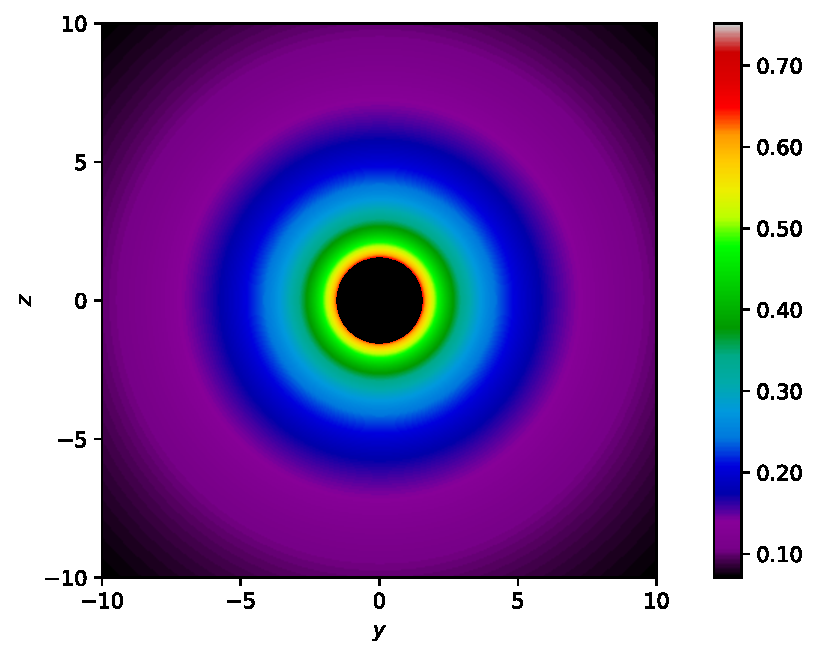
\includegraphics[width=\textwidth]{images/pdf/Rate_of_change_of_lights_velocity_field_with_respect_to_x_u_is_0.pdf}
		\caption{$\|\frac{\partial \underline{\hat{c}}}{\partial x}\|$}
		\label{fig: Rate of change of lights velocity field of rest source subfig_1}
	\end{subfigure}
	\begin{subfigure}{0.32\textwidth}
		\centering
		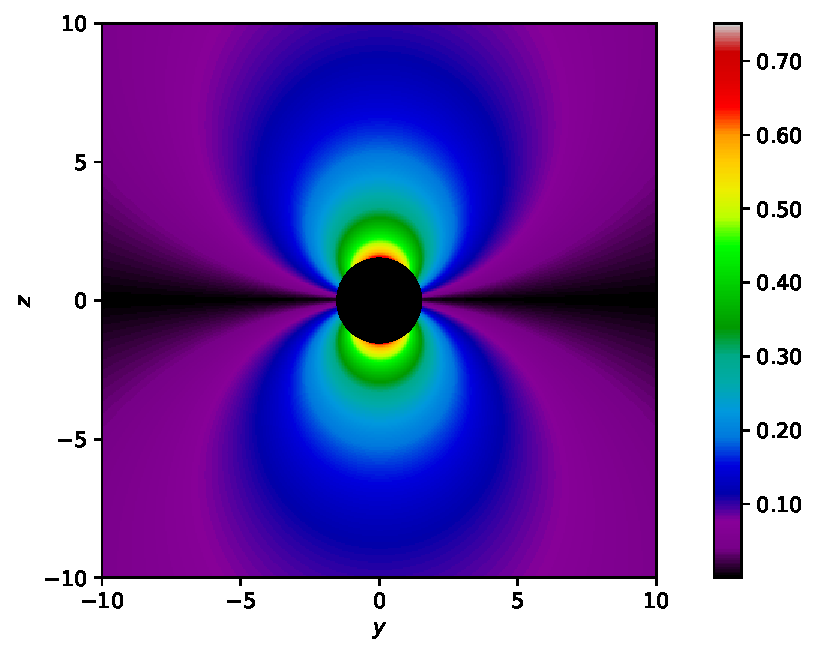
\includegraphics[width=\textwidth]{images/pdf/Rate_of_change_of_lights_velocity_field_with_respect_to_y_u_is_0.pdf}
		\caption{$\|\frac{\partial \underline{\hat{c}}}{\partial y}\|$}
		\label{fig: Rate of change of lights velocity field of rest source subfig_2}
	\end{subfigure}
	\begin{subfigure}{0.32\textwidth}
		\centering
		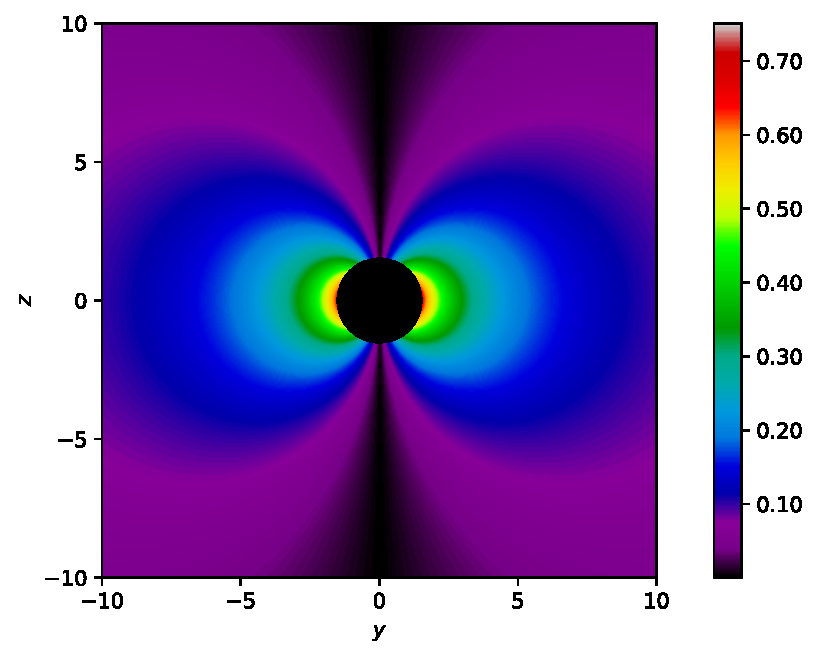
\includegraphics[width=\textwidth]{images/pdf/Rate_of_change_of_lights_velocity_field_with_respect_to_z_u_is_0.pdf}
		\caption{$\|\frac{\partial \underline{\hat{c}}}{\partial z}\|$}
		\label{fig: Rate of change of lights velocity field of rest source subfig_3}
	\end{subfigure}
	\caption{\textbf{The rate of change of the velocity vector field of light from a source at rest}. main caption.}
	\label{fig: Rate of change of lights velocity field of rest source}
\end{figure}
%███████████

%███
%█████████████
\begin{figure}[H]
	\centering
	\begin{subfigure}{0.32\textwidth}
		\centering
		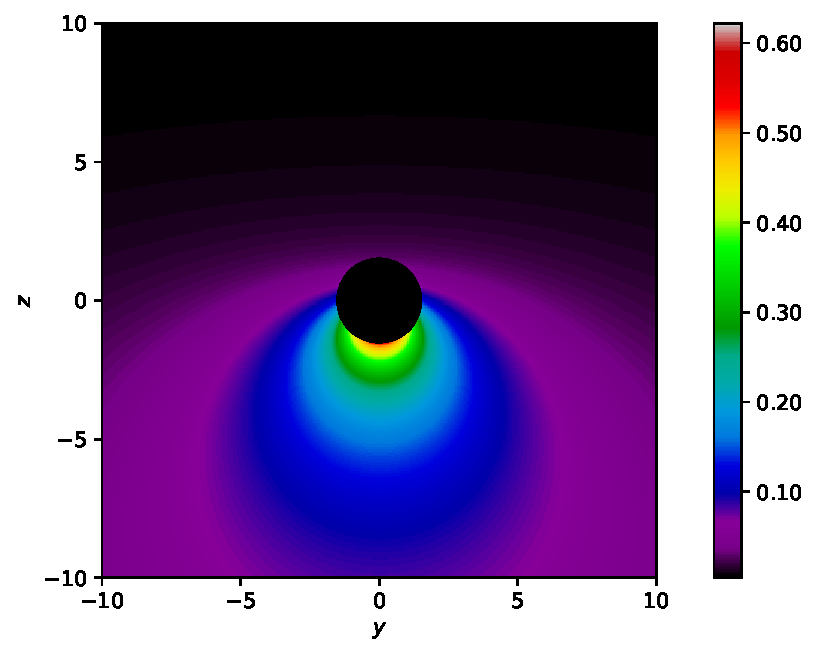
\includegraphics[width=\textwidth]{images/pdf/Rate_of_change_of_lights_velocity_field_with_respect_to_x.pdf}
		\caption{$\|\frac{\partial \underline{\hat{c}}}{\partial x}\|$}
		\label{fig: Rate of change of lights velocity field subfig_1}
	\end{subfigure}
	\begin{subfigure}{0.32\textwidth}
		\centering
		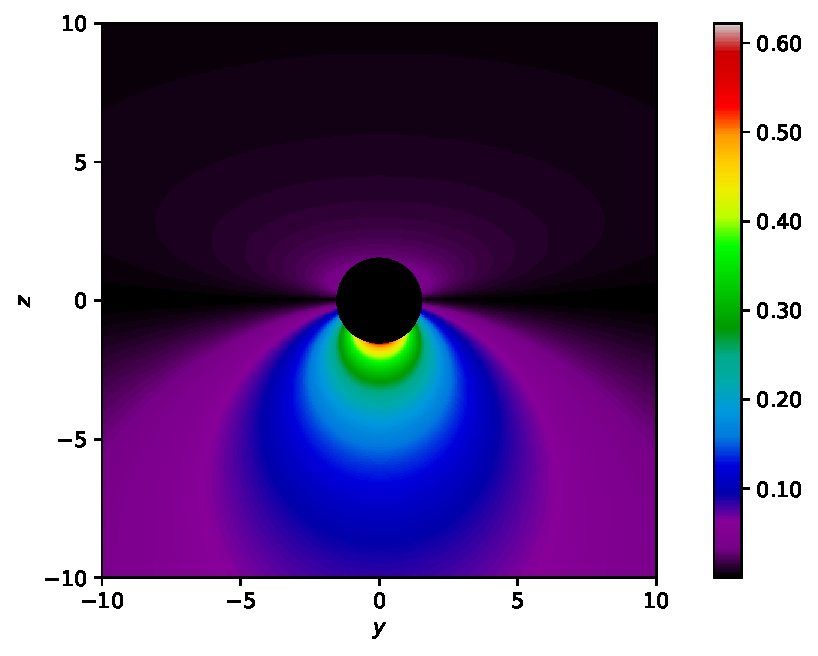
\includegraphics[width=\textwidth]{images/pdf/Rate_of_change_of_lights_velocity_field_with_respect_to_y.pdf}
		\caption{$\|\frac{\partial \underline{\hat{c}}}{\partial y}\|$}
		\label{fig: Rate of change of lights velocity field subfig_2}
	\end{subfigure}
	\begin{subfigure}{0.32\textwidth}
		\centering
		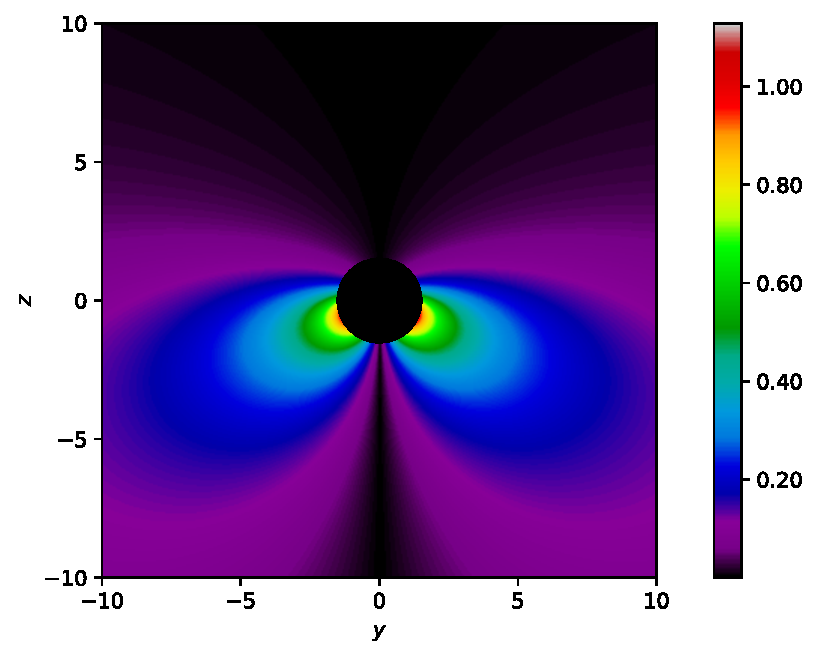
\includegraphics[width=\textwidth]{images/pdf/Rate_of_change_of_lights_velocity_field_with_respect_to_z.pdf}
		\caption{$\|\frac{\partial \underline{\hat{c}}}{\partial z}\|$}
		\label{fig: Rate of change of lights velocity field subfig_3}
	\end{subfigure}
	\caption{\textbf{The rate of change of the velocity vector field of light from a moving source}. main caption.}
	\label{fig: Rate of change of lights velocity field}
\end{figure}
%███████████

%███
%█████████████
\begin{figure}[H]
	\centering
	\begin{subfigure}{0.45\textwidth}
		\centering
		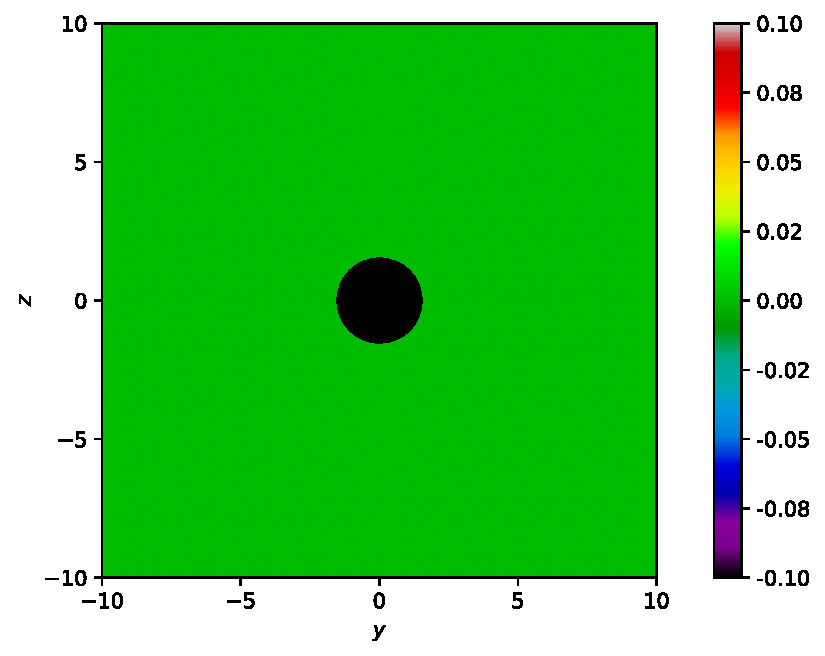
\includegraphics[width=\textwidth]{images/pdf/Rate_of_change_of_lights_velocity_field_with_respect_to_t_u_is_0.pdf}
		\caption{$\|\frac{\partial \underline{\hat{c}}}{\partial t}\|$ Source at Rest}
		\label{fig: Rate of change of lights velocity field with respect to time subfig_2}
	\end{subfigure}
	\begin{subfigure}{0.45\textwidth}
		\centering
		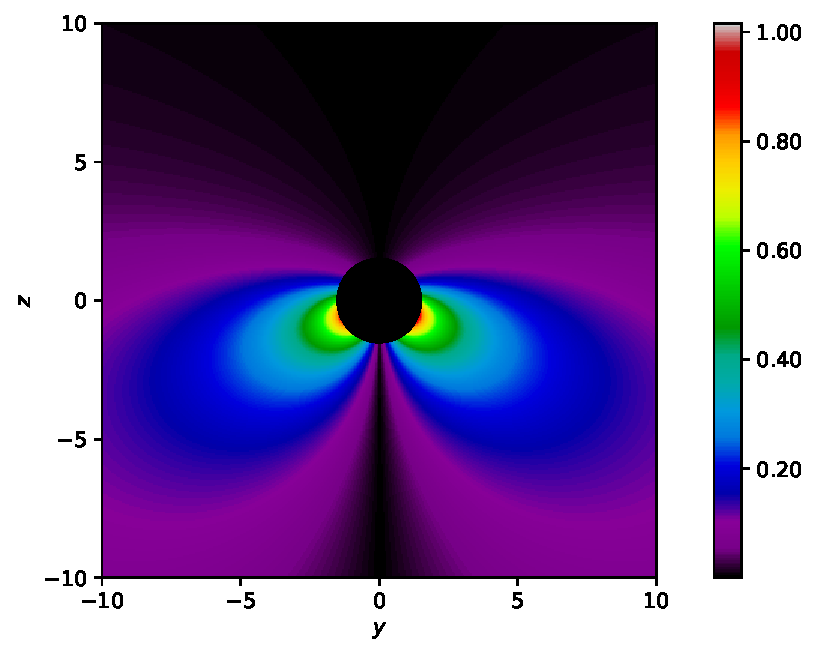
\includegraphics[width=\textwidth]{images/pdf/Rate_of_change_of_lights_velocity_field_with_respect_to_t.pdf}
		\caption{$\|\frac{\partial \underline{\hat{c}}}{\partial t}\|$ Source Moving}
		\label{fig: Rate of change of lights velocity field with respect to time subfig_3}
	\end{subfigure}
	\caption{\textbf{The rate of change of the velocity vector field of continuously emitted light from source with respect to time}. main caption.}
	\label{fig: Rate of change of lights velocity field with respect to time}
\end{figure}
%███████████

These diagrams show magnitude of the rate of change of the light's propagation direction with respect to each coordinate.

***
***

\begin{equation}
	\underline{\hat{c}} = \frac{1}{ \gamma \left( L - \beta \gamma z \right) }
		\begin{pmatrix}
			x \\
			y \\
			\gamma \left(\gamma z - \beta L \right)
		\end{pmatrix}
\end{equation}

We will use the d'Alembert operator but we will not go into its origins, but instead just note that it is lorentz



\begin{equation}
	 \square =  \frac{\partial^2}{\partial x^2} + \frac{\partial^2}{\partial y^2} + (1-\beta^2) \frac{\partial^2}{\partial z^2}
\end{equation}

The derivation of this gives a huge amount of terms, that take a long time to cancel down to a simple form, so we will just show the result of this

\begin{equation}
	  \square \underline{\hat{c}} =
	  \begin{pmatrix}
		\square \hat{c}_x \\
		\square \hat{c}_y \\
		\square \hat{c}_z
	  \end{pmatrix}
	  =
	  \frac{-2}{\gamma^2\left( 1 - \beta \frac{\gamma z}{L} \right)^2L^2} \cdot \underline{\hat{c}}
\end{equation}

***
***


We will use these to get the square root of the sum of all partial derivatives of the light's velocity, with a negative for all time derivatives, which is given by

\begin{equation}
	\sqrt{\sum_{j} \left( \frac{\partial \underline{\hat{c}}_j}{\partial x}^2 + \frac{\partial \underline{\hat{c}}_j}{\partial y}^2 + \frac{\partial \underline{\hat{c}}_j}{\partial z}^2 - \frac{\partial \underline{\hat{c}}_j}{c\partial t}^2 \right) }
\end{equation}

the reasoning for the $c$ in the time derivative is to give the derivative the same units



We will now use these differentials to get the outer product of the light's velocity field with the 4 gradient $\boldsymbol{\partial} = \left( -i\frac{\partial}{c \partial t}, \frac{\partial}{\partial x}, \frac{\partial}{\partial y}, \frac{\partial}{\partial z} \right)$ which is the extension of the gradient $\nabla=\left( \frac{\partial}{\partial x}, \frac{\partial}{\partial y}, \frac{\partial}{\partial z} \right)$ to the 4 vector.



You may ask why there is a $-i$ in front of the time derivative, this is because we are using the 4 gradient in the complex plane, and we want to keep the time derivative real, so we need to add a $-i$ to it.

You can use these differentials to get the Jacobian of the light's velocity field, which is given by

\begin{equation}
	J =
	\begin{pmatrix}
		\frac{\partial c_x}{\partial x} & \frac{\partial c_x}{\partial y} & \frac{\partial c_x}{\partial z} \\
		\frac{\partial c_y}{\partial x} & \frac{\partial c_y}{\partial y} & \frac{\partial c_y}{\partial z} \\
		\frac{\partial c_z}{\partial x} & \frac{\partial c_z}{\partial y} & \frac{\partial c_z}{\partial z} \\
	\end{pmatrix}
\end{equation}

or if you want to include the time derivative along with the 4 vector $\underline{c}= (0,c_x,c_y,c_z)$

we can take the outer product $\otimes$ of this with the 4 gradient $\boldsymbol{\partial} = \left( \frac{\partial}{c \partial t}, \frac{\partial}{\partial x}, \frac{\partial}{\partial y}, \frac{\partial}{\partial z} \right)$ which is the extention of the graient to the 4 vector

*** or argue for $\boldsymbol{\partial} = \left( i \frac{\partial}{c \partial t}, \frac{\partial}{\partial x}, \frac{\partial}{\partial y}, \frac{\partial}{\partial z} \right)$

\begin{equation}
	J =
	\begin{pmatrix}
		\frac{\partial c_t}{c\partial t} & \frac{\partial c_t}{\partial x} & \frac{\partial c_t}{\partial y} & \frac{\partial c_t}{\partial z}\\
		\frac{\partial c_x}{c \partial t} & \frac{\partial c_x}{\partial x} & \frac{\partial c_x}{\partial y} & \frac{\partial c_x}{\partial z} \\
		\frac{\partial c_y}{c \partial t} & \frac{\partial c_y}{\partial x} & \frac{\partial c_y}{\partial y} & \frac{\partial c_y}{\partial z} \\
		\frac{\partial c_z}{c \partial t} & \frac{\partial c_z}{\partial x} & \frac{\partial c_z}{\partial y} & \frac{\partial c_z}{\partial z} \\
	\end{pmatrix}
	=
	\begin{pmatrix}
		0                                 & 0                               & 0                               & 0                               \\
		-\beta\frac{\partial c_x}{\partial z} & \frac{\partial c_x}{\partial x} & \frac{\partial c_x}{\partial y} & \frac{\partial c_x}{\partial z} \\
		-\beta\frac{\partial c_y}{\partial z} & \frac{\partial c_y}{\partial x} & \frac{\partial c_y}{\partial y} & \frac{\partial c_y}{\partial z} \\
		-\beta\frac{\partial c_z}{\partial z} & \frac{\partial c_z}{\partial x} & \frac{\partial c_z}{\partial y} & \frac{\partial c_z}{\partial z} \\
	\end{pmatrix}
\end{equation}



when swaping dt with dz, we will introduce $i$ into equation, or introduce into the 4 gradient

taking the squareroot of the sum of the squares of each element in the jacobian we get ...

\begin{equation}
	\sqrt{ \sum_{i} \sum_{j}  J_{ij}^2 }
\end{equation}

% jacobian has been thouroughly checked with wolfram alpha
\begin{equation}
	\underline{J} =
	\frac{1}{\gamma  L ( 1 + \frac{u}{c} \frac{\gamma z}{L} )^2}
	\begin{pmatrix}
		\frac{y^2}{ L^2} +\left( \frac{u}{c}  + \frac{ \gamma z }{L} \right)   \frac{\gamma z}{ L}  & - \frac{xy}{L^2}  & - \gamma ( \frac{u}{c}  + \frac{ \gamma z }{L} ) \frac{x}{L} \\
		- \frac{xy}{L^2}  & \frac{x^2}{ L^2} + \left( \frac{u}{c}  + \frac{ \gamma z }{L} \right)   \frac{\gamma z}{ L}  & - \gamma (  \frac{u}{c}  + \frac{\gamma z }{L} ) \frac{y}{L}
		\\
		- \frac{xz}{L^2} & - \frac{yz}{L^2} & \frac{ x^2 + y^2 }{ L^2}
	\end{pmatrix}
\end{equation}

\begin{equation}
	\underline{J} =
	\frac{1}{\gamma  L^3 ( 1 + \frac{u}{c} \frac{\gamma z}{L} )^2}
	\begin{pmatrix}
		y^2 +\left( \frac{u}{c} L +  \gamma z \right) \gamma z  & -xy & - \gamma ( \frac{u}{c} L + \gamma z  ) x \\
		- xy  & x^2 + \left( \frac{u}{c} L  +  \gamma z \right) \gamma z  & - \gamma (  \frac{u}{c}L  + \gamma z  ) y
		\\
		- xz & - yz &  x^2 + y^2
	\end{pmatrix}
\end{equation}

% checked with wolfram alpha
\begin{equation}
	\|\underline{J}\| = \frac{\sqrt{ 2 ( x^2+ y^2 )^2 + (x^2+y^2)(M+z)^2 + 2 z^2 M^2 } }{\gamma  L^3 ( 1 + \frac{u}{c} \frac{\gamma z}{L} )^2 }
\end{equation}

$M= \gamma (  \frac{u}{c}L  + \gamma z  )$



%█████████████
\begin{figure}[H]
	\centering
	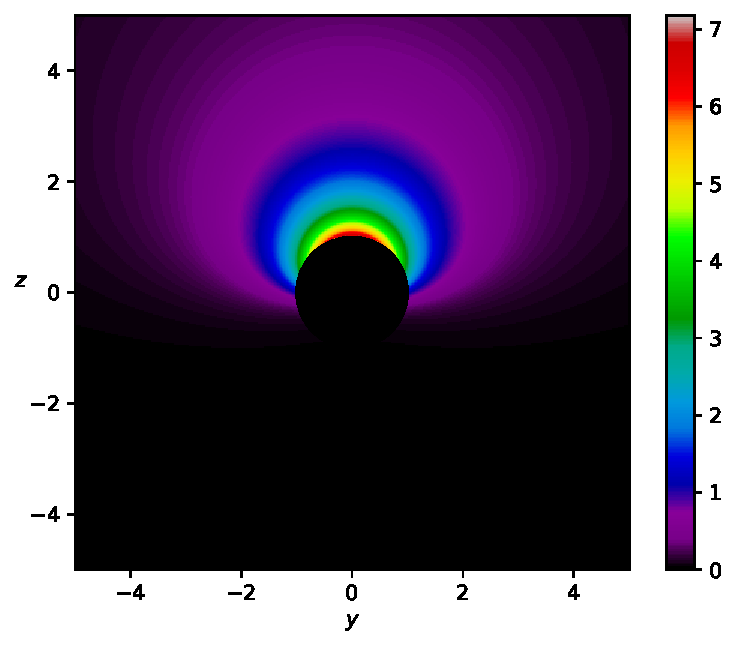
\includegraphics[width=0.9\textwidth]{images/pdf/jacobian_of_lights_velocity_norm_squared_for_Moving_Source.pdf}
	\caption{\textbf{Jacobian norm squared}. The squared norm of the Jacobian matrix of the light's velocity field for a moving source.}
	\label{fig: Jacobian norm squared}
\end{figure}
%███████████



%█████████████
\subsubsection{Alternative manipulations:}

We will use these to get the square root of the sum of all partial derivatives of the light's velocity, with a negative for all time derivatives, which is given by

\begin{equation}
	J = \sqrt{\sum_{j} \left( \frac{\partial \underline{\hat{c}}_j}{\partial x}^2 + \frac{\partial \underline{\hat{c}}_j}{\partial y}^2 + \frac{\partial \underline{\hat{c}}_j}{\partial z}^2 - \frac{\partial \underline{\hat{c}}_j}{c\partial t}^2 \right) }
\end{equation}

the reasoning for the $c$ in the time derivative is to give the derivative the same units


\begin{equation}
	\|\underline{J}\|^2 = \frac{ 2 }{\gamma^2  L^2 ( 1 - \beta \frac{\gamma z}{L} )^2 }
\end{equation}

\begin{equation}
	\left\| \nabla \|\underline{J}\| \right\|
	= - \frac{ \sqrt{2} }{ L^2 ( 1 - \beta \frac{\gamma z}{L}) }
\end{equation}

\begin{equation}
	\nabla \|\underline{J}\| \cdot \hat{\underline{c}} =  \frac{ \sqrt{2} }{ L^2 ( 1 - \beta \frac{\gamma z}{L} ) }
\end{equation}

jacobian with time components, with $m= \gamma (  -\beta L  + \gamma z  )$

\begin{equation}
	\|\underline{J}_t\| = \frac{ \sqrt{(x^2+y^2)^2 + \frac{L^2}{\gamma^2}(x^2+y^2) +2m^2z^2 + (x^2+y^2)(2mz +\frac{m^2}{\gamma^2}) }}{\gamma  L^3 ( 1 - \beta \frac{\gamma z}{L} )^2 }
\end{equation}

\begin{equation}
	m = \gamma (  \gamma z - \beta L ) = L \gamma (T-\beta)
\end{equation}

$T=\frac{\gamma z}{L}$

lets look at

\begin{equation}
	\begin{aligned}
		W &= (x^2+y^2)^2 + \frac{L^2}{\gamma^2}(x^2+y^2) +2m^2z^2 + (x^2+y^2)(2mz +\frac{m^2}{\gamma^2})
		\\
		&= (L^2 -\gamma^2z^2)^2 + \frac{L^2}{\gamma^2}(L^2 -\gamma^2z^2) +2 L^2 \gamma^2z^2 (T-\beta)^2 + (L^2 -\gamma^2z^2)(2 L \gamma z (T-\beta) + L^2 (T-\beta)^2) \\
		&= L^4 \left[ (1-T^2)^2 + (1-\beta^2)(1-T^2) +2T^2 (T-\beta)^2 + (1 - T^2)(2 T (T-\beta) + (T-\beta)^2)  \right]
		\\
		& \text{wolfram alpha gives} \\
		&= 2 L^4 (1- \beta T)^2
	\end{aligned}
\end{equation}

then

\begin{equation}
	\|\underline{J}_t\| = \frac{ \sqrt{ 2 L^4 (1- \beta \frac{\gamma z}{L})^2 }}{\gamma  L^3 ( 1 - \beta \frac{\gamma z}{L} )^2 }
\end{equation}

\begin{equation}
	\|\underline{J}_t\| = \frac{ \sqrt{2} }{\gamma  L ( 1 - \beta \frac{\gamma z}{L} ) } = \frac{ \sqrt{2} }{\gamma  ( L - \beta \gamma z ) }
\end{equation}

\begin{equation}
	\|\underline{J}_t\|^2 = \frac{ 2 }{\gamma^2  L^2 ( 1 - \beta \frac{\gamma z}{L} )^2 }
\end{equation}

for gradient:

\begin{equation}
	\partial_x \|\underline{J}_t\|  = - \frac{ \sqrt{2} x }{\gamma L ( L - \beta \gamma z )^2 }
\end{equation}

\begin{equation}
	\partial_y \|\underline{J}_t\|  = - \frac{ \sqrt{2} y }{\gamma L ( L - \beta \gamma z )^2 }
\end{equation}

\begin{equation}
	\partial_z \|\underline{J}_t\|  = - \frac{ \sqrt{2} \gamma (\gamma z - \beta L) }{\gamma L ( L - \beta \gamma z )^2 }
\end{equation}

$- u dt = dz $ so $dt = - \frac{dz}{u}$ giving

\begin{equation}
	\frac{d}{c dt} \|\underline{J}_t\|  = - \beta \frac{d}{ dz} \|\underline{J}_t\|
\end{equation}

\begin{equation}
	\nabla \|\underline{J}_t\| = - \frac{ \sqrt{2} }{\gamma L ( L - \beta \gamma z )^2 }
	\begin{pmatrix}
		x \\
		y \\
		\gamma (\gamma z - \beta L)
	\end{pmatrix}
\end{equation}

\begin{equation}
	\begin{aligned}
	\nabla \|\underline{J}_t\| \cdot \hat{\underline{c}} &=  - \frac{ \sqrt{2} }{\gamma L ( L - \beta \gamma z )^2 }
	\begin{pmatrix}
		x \\
		y \\
		\gamma (\gamma z - \beta L)
	\end{pmatrix}
	\cdot
	\frac{1}{ \gamma \left( L - \beta \gamma z \right) }
		\begin{pmatrix}
			x \\
			y \\
			\gamma \left(\gamma z - \beta L \right)
		\end{pmatrix} \\
	&= \sqrt{2} \frac{ x^2+y^2 + \gamma^4z^2-2\gamma^3\beta Lz + \beta^2\gamma^2L^2}{ L \gamma^2  ( L - \beta \gamma z )^3 } \\
	&= \sqrt{2} \frac{ L^2 - \gamma^2z^2 + \gamma^4z^2-2\gamma^3\beta Lz + \beta^2\gamma^2 L^2}{ L^4 \gamma^2  ( 1 - \beta \frac{\gamma z }{L} )^3 } \\
	&= \sqrt{2} \frac{ (\gamma^2-1) \frac{\gamma^2 z^2}{L^2} -2\gamma^2\beta \frac{\gamma z}{L} + (\beta^2\gamma^2 + 1 )}{ L^2 \gamma^2  ( 1 - \beta \frac{\gamma z }{L} )^3 } \\
	&= \sqrt{2} \frac{ \beta^2\gamma^2 T^2 -2\gamma^2\beta T + \gamma^2 }{ L^2 \gamma^2  ( 1 - \beta T )^3 } \\
	&= \sqrt{2} \frac{ (\beta\gamma T - \gamma)^2 }{ L^2 \gamma^2  ( 1 - \beta T )^3 } \\
	&= \sqrt{2} \frac{ \gamma^2(1-\beta T)^2 }{ L^2 \gamma^2  ( 1 - \beta T )^3 } \\
	&=  \frac{ \sqrt{2} }{ L^2 ( 1 - \beta T ) }
	\end{aligned}
\end{equation}

\begin{equation}
		\gamma^2 = 1+\beta^2\gamma^2,
\end{equation}

\begin{equation}
		\gamma^2 - 1 = \beta^2\gamma^2,
\end{equation}

\begin{equation}
	\left\| \nabla \|\underline{J}_t\| \right\|
	= - \frac{ \sqrt{2} }{ L^2 ( 1 - \beta \frac{\gamma z}{L}) }
\end{equation}

...

diff equals

\begin{equation}
	\begin{aligned}
	\partial_x \| J\| &= \frac{(3L-\beta\gamma z)x}{\gamma L^3(\beta\gamma z - L)^3} \cdot \sqrt{ 2 ( x^2+ y^2 )^2 + (x^2+y^2)(M+z)^2 + 2 z^2 M^2 } +  \\
	& \frac{1}{\gamma L^3 (1-\beta\frac{\gamma z}{L})^2} \cdot
	\end{aligned}
\end{equation}

\begin{equation}
	\begin{aligned}
	\partial_y \| J\| &= \frac{(3L-\beta\gamma z)y}{\gamma L^3(\beta\gamma z - L)^3} \cdot \sqrt{ 2 ( x^2+ y^2 )^2 + (x^2+y^2)(M+z)^2 + 2 z^2 M^2 } +  \\
	& \frac{1}{\gamma L^3 (1-\beta\frac{\gamma z}{L})^2} \cdot
	\end{aligned}
\end{equation}

\begin{equation}
	\begin{aligned}
	\partial_z \| J\| &= \frac{(3L-\beta\gamma z)\gamma z - 2\beta L^2}{ L^3(\beta\gamma z - L)^3} \cdot \sqrt{ 2 ( x^2+ y^2 )^2 + (x^2+y^2)(M+z)^2 + 2 z^2 M^2 } +  \\
	& \frac{1}{\gamma L^3 (1-\beta\frac{\gamma z}{L})^2} \cdot
	\end{aligned}
\end{equation}

$f=\sqrt{u}$

$u=2 ( x^2+ y^2 )^2 + (x^2+y^2)(M+z)^2 + 2 z^2 M^2 $

$\frac{df}{dx}=\frac{df}{du}\cdot \frac{du}{dx}$

\begin{equation}
	\frac{df}{dx} = \frac{1}{2\sqrt{u}} \cdot \frac{du}{dx}
\end{equation}

\begin{equation}
	\frac{du}{dx} = 2x \left( \beta^2 \gamma^2 (\gamma^2z^2 +2r^2) - \beta \gamma \frac{z}{L} \left( 3(\gamma^2+1)(x^2+y^2) + 2(\gamma^2+2)\gamma^2z^2 \right) + (\gamma^2+1)^2z^2 + 4(x^2+y^2) \right)
\end{equation}

\begin{equation}
	\frac{du}{dy} = 2y \left( \beta^2 \gamma^2 (\gamma^2z^2 +2r^2) - \beta \gamma \frac{z}{L} \left( 3(\gamma^2+1)(x^2+y^2) + 2(\gamma^2+2)\gamma^2z^2 \right) + (\gamma^2+1)^2z^2 + 4(x^2+y^2) \right)
\end{equation}

\begin{equation}
	\frac{du}{dz} = 4\gamma^2 z (\gamma z -\beta L) \left( \gamma z(1-\beta\frac{\gamma z}{L}) + (\gamma z -\beta L) \right) +
	2(x^2+y^2)(\gamma^2+1-\beta\gamma^3\frac{z}{L})(-\beta\gamma L + (\gamma^2+1)z )
\end{equation}


% we can check do see if we take the dot product of the lights velocity with the rate of change that we get a value of zero, as the two vectors should be perpendicular, which we do:

% \begin{equation}
% 	\underline{\hat{c}}' \cdot \frac{\partial \underline{\hat{c}}'}{\partial x'} = l_x' (1 - \frac{l_x'^2}{ L^2} + \frac{u}{c}\frac{\gamma l_z'}{L}) + l_y' (- \frac{l_x'}{L} \frac{l_y'}{L}) + (\gamma^2 l_z' + \gamma \frac{u}{c}  L)(- \frac{l_x'}{L} \frac{l_z'}{L})=0
% \end{equation}

% \begin{equation}
% 	\underline{\hat{c}}' \cdot \frac{\partial \underline{\hat{c}}'}{\partial z'} = l_x' (( - \frac{u}{c}  - \frac{ \gamma l_z' }{L} ) \frac{l_x'}{L}) + l_y' (( - \frac{u}{c}  - \frac{\gamma l_z' }{L} ) \frac{l_y'}{L}) + (\gamma^2 l_z' + \gamma \frac{u}{c}  L)(\frac{1}{\gamma}\frac{ l_x'^2 + l_y'^2 }{ L^2})=0
% \end{equation}

The Magnitude of this Jacobian is messy so I will not write it out here, as it would serve no purpose.
Also unsure wether to include the time derivate into the Jacobian to make it a 4 by 4 tensor like below, using the velocity $( 0 , c_x , c_y , c_z )$ (with the zero representing the derivatives of time), giving

\begin{equation}
	J =
	\begin{pmatrix}
		0                                 & 0                               & 0                               & 0                               \\
		\frac{\partial c_x}{c \partial t} & \frac{\partial c_x}{\partial x} & \frac{\partial c_x}{\partial y} & \frac{\partial c_x}{\partial z} \\
		\frac{\partial c_y}{c \partial t} & \frac{\partial c_y}{\partial x} & \frac{\partial c_y}{\partial y} & \frac{\partial c_y}{\partial z} \\
		\frac{\partial c_z}{c \partial t} & \frac{\partial c_z}{\partial x} & \frac{\partial c_z}{\partial y} & \frac{\partial c_z}{\partial z} \\
	\end{pmatrix}
\end{equation}

But instead of going through this, I will end the madness of this chapter here and move on to looking at quantities that do not change when swaping frames, which will lead to the famous energy-mass and energy-momentum equations.

\begin{equation}
	\big\| \nabla \|\underline{J}\| \big\| = \frac{\sqrt{2}}{r^2}
\end{equation}

*** also try direction derivative of the Jacobian norm $ \nabla \|\underline{J}\| \cdot \hat{\underline{c}}$

I have however exhausted the different ways that I thought were reasonable avenues to check. apart from a property called the material derivative, given as

\begin{equation}
	\rho {\frac {\mathrm {D} \underline {u} }{\mathrm {D} t}}=\rho \left({\frac {\partial \underline {u} }{\partial t}}+(\underline {u} \cdot \nabla )\underline {u} \right)
\end{equation}

which when the normal is taken you get $1/r$, but I shall not got through this here as its a bit too much.


% gradient being $( \delta_t , \delta_x , \delta_y , \delta_z )$



%for norm should above have negative time parts? or make complex?

%███████████████████████████████████████████████████████████████████
%███████████████████████████████████████████████████████████████████
%███████████████████████████████████████████████████████████████████
\chapter{Force from a Current Carrying Wire}\label{sect: Force from a Current Carrying Wire}

*** i think the electrons will be spread out by a factor of gamma in lab frame but the quantity i will use will make up for the gamma factor

*** these tikz will have errors when using script
\newcommand{\Nval}{10}
%█████████████
\begin{figure}[H]
	\centering
	\begin{subfigure}{\textwidth}
		\centering
		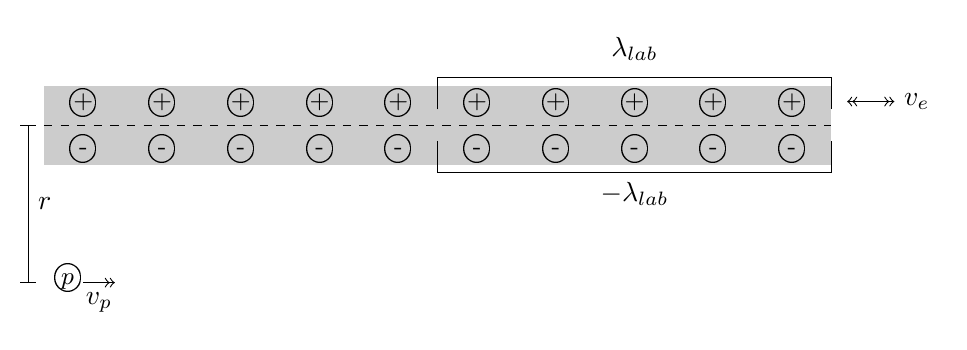
\begin{tikzpicture}
			\fill [gray!40] (0,-0.5) rectangle (\Nval,0.5);
			\draw[black, dashed,-] (0,0) -- (\Nval,0);
			\foreach \x in {0,1,...,\numexpr\Nval-1\relax}{ % Loop from 0 to Nval-1
					\node at (\x+0.5,0.25){\textcircled{\small{+}}};
				};
			\foreach \x in {0,1,...,\numexpr\Nval-1\relax}{ % Loop from 0 to Nval-1
					\node at (\x+0.5,-0.35){\textcircled{\small{-}}};
				};
			\draw[black] (5,0.2) -- (5,0.6) -- (10,0.6) -- (10,0.2);
			\draw[draw=none] (5,0.6) -- (10,0.8) node[midway,above]{$\lambda_{lab}$};
			\draw[black] (5,-0.2) -- (5,-0.6) -- (10,-0.6) -- (10,-0.2);
			\draw[draw=none] (5,-0.6) -- (10,-0.6) node[midway,below]{$-\lambda_{lab}$};
			\draw[<<->>] (\Nval+0.2,0.3) -- (\Nval+0.8,0.3) node[right]{$v_e$}; % Using Nval here
			\draw[|-|] (-0.2,0) -- (-0.2,-2) node[midway,right]{$r$};
			\node at (0.3,-2) {\textcircled{\small{$p$}}};
			\draw[->>] (0.5,-2) -- (0.9,-2) node[midway,below]{$v_p$};
		\end{tikzpicture}
		\caption{lab frame}
		\label{subfig_1: current in a wire}
	\end{subfigure}
	\begin{subfigure}{\textwidth}
		\centering
		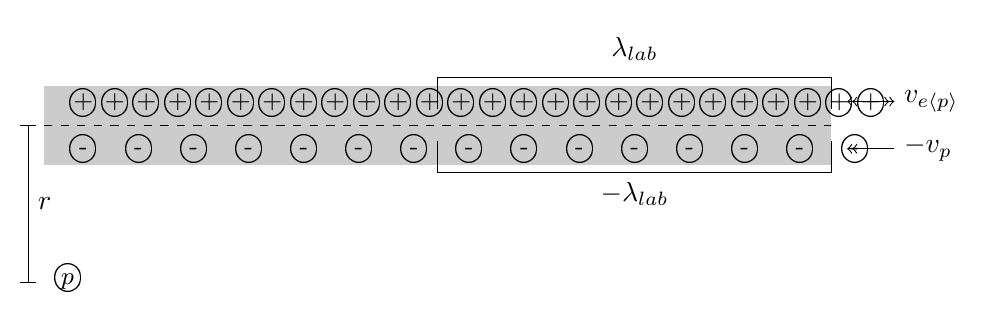
\begin{tikzpicture}
			\fill [gray!40] (0,-0.5) rectangle (\Nval,0.5);
			\draw[black, dashed,-] (0,0) -- (\Nval,0);
			\foreach \x in {0,0.4,...,\Nval}{ % Using Nval for the upper limit
					\node at (\x+0.5,0.25){\textcircled{\small{+}}};
				};
			\foreach \x in {0,0.7,...,\Nval}{ % Using Nval for the upper limit
					\node at (\x+0.5,-0.35){\textcircled{\small{-}}};
				};
			\draw[black] (5,0.2) -- (5,0.6) -- (10,0.6) -- (10,0.2);
			\draw[draw=none] (5,0.6) -- (10,0.8) node[midway,above]{$\lambda_{lab}$};
			\draw[black] (5,-0.2) -- (5,-0.6) -- (10,-0.6) -- (10,-0.2);
			\draw[draw=none] (5,-0.6) -- (10,-0.6) node[midway,below]{$-\lambda_{lab}$};
			\draw[<<->>] (\Nval+0.2,0.3) -- (\Nval+0.8,0.3) node[right]{$v_{e \langle p \rangle}$}; % Using Nval here
			\draw[<<-] (\Nval+0.2,-0.3) -- (\Nval+0.8,-0.3) node[right]{$-v_p$}; % Using Nval here
			\draw[|-|] (-0.2,0) -- (-0.2,-2) node[midway,right]{$r$};
			\node at (0.3,-2) {\textcircled{\small{$p$}}};
		\end{tikzpicture}
		\caption{charge frame}
		\label{subfig_2: current in a wire}
	\end{subfigure}
	\caption{\textbf{current in a wire}. main caption.}
	\label{fig: current in a wire}
\end{figure}
%███████████



\begin{figure}[H]
	\centering
	\begin{tikzpicture}[>=latex]
		\fill [gray!40] (-0.1,-0.5) rectangle (0.1,3);
		\fill [blue!60] (-0.1,1.3) rectangle (0.1,1.7)node[midway, left] {$dl$};
		\draw[->,thick,dashed,black] (0,1.5) -- (0:4) node[midway, above] {$\vec{r}$};
		\draw[->,thick,black] (0,0) -- (0:5) node [below] {$Y$};
		\draw[->,thick,black] (0,0) -- (90:2.5) node [left] {$Z$};
		\draw[->,dashed,black] (4,0) -- (4,2.5) node [right] {$\vec{v}$};
		\draw[|-|,black] (-0.6,0) -- (-0.6,1.5) node [midway, left] {$l$};
		\draw[|-|,black] (0,-0.25) -- (4,-0.25) node [midway,below] {$d$};
		\draw[-,dashed,black] (0,-0.5) -- (0,3);
		\fill [blue] (4,0) circle (3pt) node[above right] {$P$};
		\draw [->,red, dashed,thick ] (0,2.2) arc (90:-20:0.7cm)    node [midway, right] {$\theta$};
		\draw [thick] (0,0.8) arc (-90:-20:0.7cm) node [midway, below] { \ \ $\pi-\theta$};
		\draw [thick] (4,0.7) arc (90:160:0.7cm) node [midway, above] {\hspace{-0.5cm}$\pi-\theta$};
		\node at (8,2) {$\cos{(\pi-\theta)}=-\cos{\theta}$};
		\node at (8,1) {$\cos{\theta}= \dfrac{-l}{\sqrt{d^2+l^2}}$};
	\end{tikzpicture}
	\caption{lab frame}
\end{figure}

\begin{equation}
	\vec{r} = \begin{pmatrix}
		0 \\ d \\ -l
	\end{pmatrix}
	= \begin{pmatrix}
		0 \\ d \\ \dfrac{d}{\tan\theta}
	\end{pmatrix}
\end{equation}

%███████████████████████████████████████████████████████████████████
%███████████████████████████████████████████████████████████████████
\section{stationary charge}\label{sect: stationary charge}

\textbf{lab frame:}

$u_e$ is electron's speed

$u_r=0$ is recieving charges speed

$u_i = 0$ is ions speed

charge position $(y,0)$

any particular electrons location given by at $(0,z)$ at time $t=0$

the retarded time of electron is given by

\begin{equation}
	T_{ret} = - \gamma_{u_e}^2\frac{u_e}{c^2} l_{z} - \frac{\gamma_{u_e}}{c}\sqrt{ l_{y}^2+\gamma_{u_e}^2 l_{z}^2}
\end{equation}


*** $(l_y,l_z)$ is the position of the receiving charge relative to the electron's retarded position, so $(l_y,l_z)= (y,-z)$

relative retarded position from $z$ is $u_e T_{ret}$

\begin{equation}
z_{ret} - z = \gamma_{u_e}^2\frac{u_e^2}{c^2} z - \gamma_{u_e}\frac{u_e}{c}\sqrt{ y^2+\gamma_{u_e}^2 z^2}
\end{equation}

actual retarded position is this + z

\begin{equation}
z_{ret} = (1+\gamma_{u_e}^2\frac{u_e^2}{c^2}) z - \gamma_{u_e}\frac{u_e}{c}\sqrt{ y^2+\gamma_{u_e}^2 z^2}
\end{equation}

\begin{equation}
z_{ret} = \gamma_{u_e}^2 z - \gamma_{u_e}\frac{u_e}{c}\sqrt{ y^2+\gamma_{u_e}^2 z^2}
\end{equation}

\begin{equation}
z_{ret} = \gamma_{u_e} \left(\frac{\gamma_{u_e} z}{\sqrt{ y^2+\gamma_{u_e}^2 z^2}} - \frac{u_e}{c} \right) \sqrt{ y^2+\gamma_{u_e}^2 z^2}
\end{equation}

the density of the retarded positions of the charges are given by (from gemini, need to check)

\begin{equation}
\lambda_{ret} = \left( 1 + \frac{u_e}{c}\frac{z}{\sqrt{ y^2+ z^2}} \right)\lambda
\end{equation}

*** think this should have a gamma infront of each Z

as should be diferentiating with respect to dz instead of $dz_{ret}$ and change is bigger than change in dz, and we want change in dz i think
